\UseRawInputEncoding
%% Proxy4Tun — Automation in Construction (cas-dc double-column template)

\documentclass[a4paper,fleqn]{cas-dc}

\usepackage[numbers]{natbib}
\usepackage{booktabs}
\usepackage{multirow}
\usepackage{amsmath}
\usepackage{algorithm}
\usepackage{algpseudocode}
\usepackage{graphicx}
\usepackage[dvipsnames]{xcolor}
% Better line breaks for long URLs (esp. in two-column bibliographies)
\usepackage{xurl}
\usepackage{hyperref}
% Clever cross-references (\cref, \Cref). Must be loaded after hyperref.
\usepackage[nameinlink,noabbrev]{cleveref}
\usepackage{placeins}
\usepackage{caption}
\usepackage{subcaption}
\usepackage{balance}
\usepackage[normalem]{ulem}
\usepackage[most]{tcolorbox} % for section-wide highlighting

\providecommand{\printorcid}{}
\providecommand{\printfacebook}{}
\providecommand{\printtwitter}{}
\providecommand{\printlinkedin}{}
\providecommand{\printgplus}{}
\providecommand{\printinstagram}{}
\providecommand{\printemails}{}
\providecommand{\printurls}{}
\usepackage{lineno} % line numbers
% \linenumbers % (enabled below after \maketitle)

\begin{document}
\let\WriteBookmarks\relax
\def\floatpagepagefraction{1}
\def\textpagefraction{.001}



% ────────────────────────────── Front matter ──────────────────────────────

\shorttitle{Proxy4Tun: deployment-label-free tunnel lining segmentation}
\shortauthors{X.\ Tao et~al.}

\title[mode=title]{Proxy4Tun: proxy-driven deployment-label-free segmental tunnel lining segmentation}

\author[1]{Xinghui Tao}
\credit{Conceptualization, Methodology, Software, Writing -- original draft}

\author[2]{Zehao Ye}


\author[1]{Guangming Wang}
\cormark[1]
\ead{gw462@cam.ac.uk}
\credit{Supervision, Writing -- review \& editing}

\author[2]{Jelena Nini\'{c}}
\credit{Supervision, Writing -- review \& editing}

\author[1]{Brian Sheil}
\credit{Supervision, Funding acquisition, Project administration}

\cortext[cor1]{Corresponding author}

\affiliation[1]{organization={Construction Engineering, University of Cambridge},
    addressline={Trumpington Street},
    city={Cambridge},
    postcode={CB2 1PZ},
    country={United Kingdom}}

\affiliation[2]{organization={Department of Engineering, Durham University},
    addressline={Stockton Road},
    city={Durham},
    postcode={DH1 3LE},
    country={United Kingdom}}

% ─── Abstract ─────────────────────────────────────────────────────────────


\begin{abstract}
Automated inspection of segmental tunnel linings requires accurate point-cloud segmentation, yet deployment rarely provides ground-truth (GT) labels for retuning or quality control: without labels, the system must still decide whether to accept, refine, or flag each result. This paper presents Proxy4Tun, a framework that estimates segmentation quality without deployment labels. At design time, Bayesian-optimisation (BO) exploration of the bounded parameter space around one expert-tuned anchor per lining family is used as an experience generator: 40 labelled trials per family (120 in total, all six pipeline stages tunable) deliberately span healthy to degraded configurations. Feature ablation over GT-free \emph{evidence} and \emph{coherence} metrics distils this experience into a frozen five-feature Ridge proxy with a calibrated low-quality alarm. At deployment, the proxy predicts mean Intersection-over-Union (mIoU) from intermediate pipeline artifacts alone, requiring only a family declaration and the segments-per-ring count. On 27 held-out Seg2Tunnel subsets (54 scored runs), the frozen proxy attains Spearman rank correlation 0.848 and mean absolute error 0.071, ranks the anchor above a known-bad configuration on 27/27 subsets, and flags all 27 known-bad runs with zero false alarms. A proof-of-concept self-refinement loop that selects LLM-proposed parameter overlays by proxy score improves mIoU on four of five subsets (gains $+$0.040 to $+$0.353). These results support calibrated intrinsic proxies as auditable, label-free control signals for tunnel-lining segmentation pipelines.
\end{abstract}


% ─── Highlights ───────────────────────────────────────────────────────────

\begin{highlights}
\item Propose Proxy4Tun for label-free quality estimation of tunnel-lining segmentation.
\item Distil Bayesian-exploration trials into a frozen five-feature GT-free mIoU proxy.
\item Achieve Spearman 0.848 and MAE 0.071 on 27 held-out subsets.
\item Flag all 27 known-bad runs with zero false alarms.
\item Proxy-selected self-refinement improves mIoU on four of five subsets.
\end{highlights}

% ─── Keywords ─────────────────────────────────────────────────────────────

\begin{keywords}
Segmental tunnel lining \sep Point cloud segmentation \sep Deployment quality control \sep Intrinsic proxy \sep Bayesian optimisation \sep Reflective LLM agents
\end{keywords}
\date{\today}

\maketitle
\linenumbers

\smallskip
% ─────────────────────────────────────────────────────────────────────────

% ══════════════════════════════════════════════════════════════════════════
\section{Introduction}\label{sec:intro}
% ══════════════════════════════════════════════════════════════════════════

Automated inspection of segmental tunnel linings is required to support structural health assessment and long-term operational safety, given the scale, frequency, and access constraints of modern tunnel networks~\cite{attard2018,montero2015,strauss2020sensing}. Modern laser scanning enables high-fidelity tunnel capture, but the resulting measurements contain mixed structural elements, occlusions, and noise, and lining geometry, layout, and acquisition settings vary from project to project~\cite{huang2021bim,sjolander2023towards,weidner2024generalized,yue2024damage}. In practice, a deployed segmentation system must therefore do more than segment: without ground-truth (GT) labels it must also decide whether each result should be \emph{accepted}, \emph{refined}, or \emph{flagged} for review (Fig.~\ref{fig:deployment_qc_gap}).

\begin{figure*}[t]
\centering
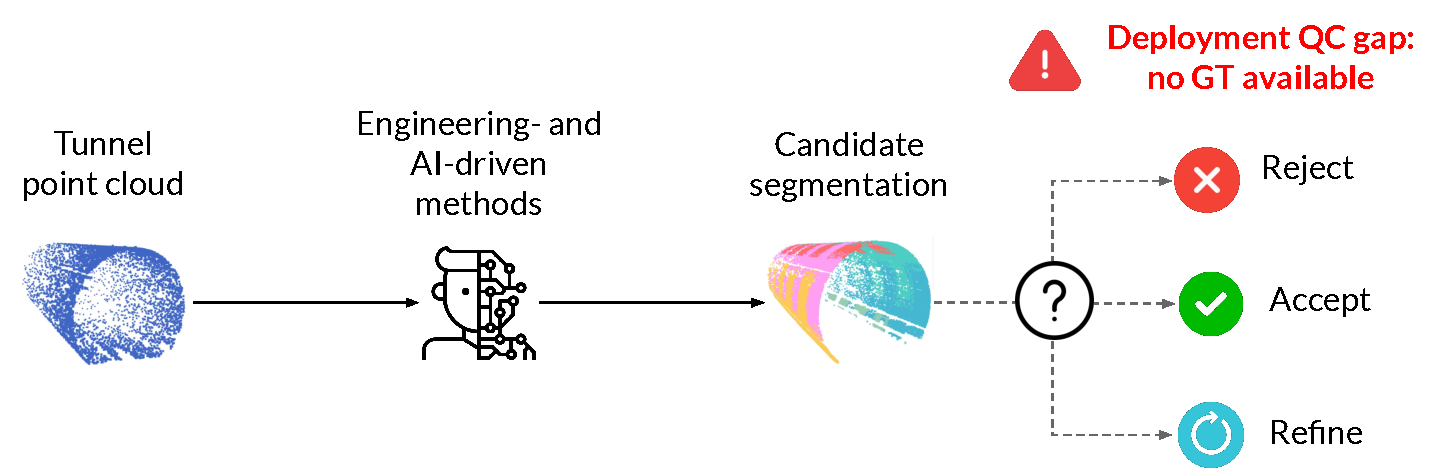
\includegraphics[width=0.8\textwidth]{figs/motivation.pdf}
\caption{Deployment quality-control (QC) gap: both engineering-driven and AI-driven tunnel-segmentation methods produce candidate outputs, but without ground-truth (GT) at deployment they lack a direct mechanism for deciding whether each result should be rejected, accepted, or refined.}
\label{fig:deployment_qc_gap}
\end{figure*}

Existing tunnel point-cloud methods span three broad families. Engineer-designed geometric pipelines fit centrelines, unroll surfaces, and apply density or curvature rules; their logic is auditable but brittle when diameter, joint pattern, or point density change~\cite{weidner2024generalized,huang2021bim,wang2025automated}. Supervised deep networks---general point-cloud backbones~\cite{qi2017pointnet,hu2020randla,schult2023mask3d,kolodiazhnyi2024td3d} and tunnel-specific models~\cite{duan2023high,su2024review,cha2024deep,wang2026serialformer}---adapt through data but require large labelled corpora and periodic retraining, which deployment rarely provides. Foundation-model pipelines bypass per-project annotation by prompting models pre-trained at scale~\cite{bommasani2021foundation,kirillov2023sam,ye2024sam}; among them, SAM4Tun~\cite{ye2025sam4tun} combines point-cloud preprocessing with SAM-based prompting and achieves strong accuracy under expert tuning, but exposes dozens of processing parameters that do not transfer when conditions depart from the tuning reference. LLM-guided adapters can retune such parameters from structured context, yet they leave open the deployment-control question: \emph{how should the system know, without GT, that a candidate configuration is acceptable?} Label-free quality-control scores from medical and general vision---reverse classification accuracy and related checks~\cite{valindria2017rca,robinson2018segmentationQuality,fournel2021segmentationQC}---are not specialised to the failure modes of cylindrical tunnel unfolding (orientation collapse, hollow evidence, circumferential phase errors) and do not expose an engineer-auditable accept/refine/flag decision tied to pipeline stages (Fig.~\ref{fig:conceptual_positioning}).

\begin{figure*}[t]
\centering
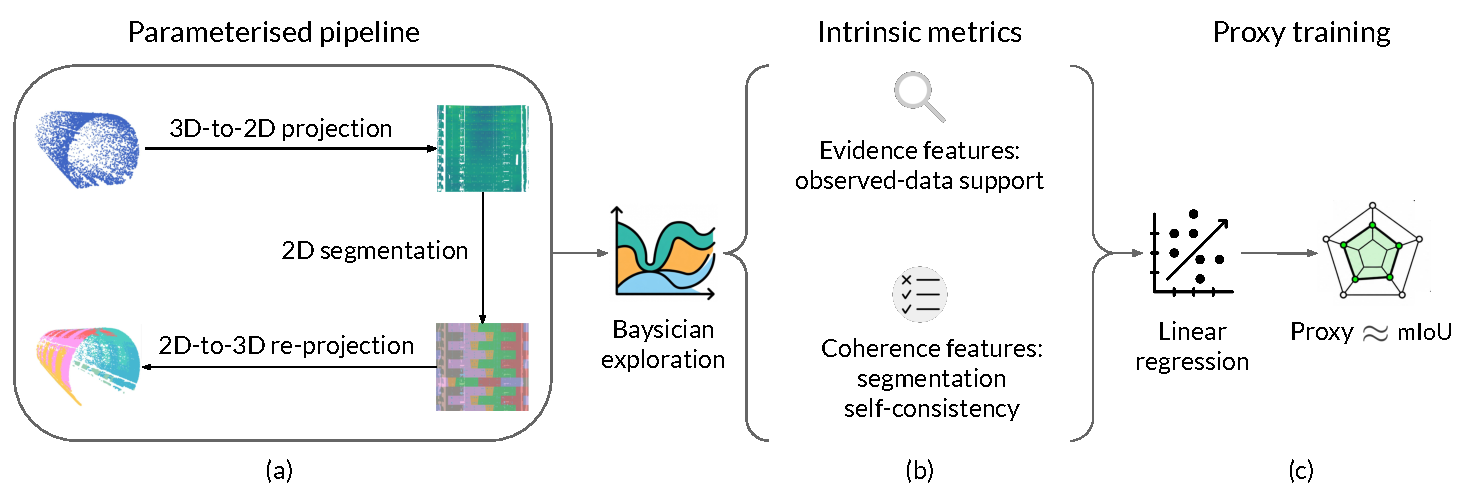
\includegraphics[width=1\textwidth]{figs/intrinsics.pdf}
\caption{Proxy4Tun: design-time construction of a GT-free intrinsic proxy for deployment-time QC. (a) A parameterised pipeline (3D$\rightarrow$2D projection, 2D segmentation, 2D$\rightarrow$3D re-projection) is exercised via Bayesian exploration to generate diverse high/low-quality trials. (b) Each trial is summarised by intrinsic GT-free features: \emph{evidence} (observed-data support) and \emph{coherence} (segmentation self-consistency). (c) A linear regressor maps these features to a scalar proxy score, calibrated offline to estimate GT mIoU so high scores indicate reliable segmentations, while low scores are flagged for rejection or refinement without requiring GT at deployment. (\textit{Note:} parameterisation, Bayesian exploration, and the linear-regression details are described in Section~\ref{sec:methods}.)}
\label{fig:intrinsic_proxy_scoring}
\end{figure*}

Proxy4Tun addresses this gap for a fixed, unified SAM4Tun stage graph (Fig.~\ref{fig:intrinsic_proxy_scoring}). Design-time Bayesian-optimisation (BO) exploration around one expert-tuned anchor per lining family is used purely as an \emph{experience generator}, not as the final optimisation engine: 40 space-filling trials per family (120 in total, with all six pipeline stages tunable) deliberately span healthy to degraded configurations so that GT-free intrinsic metrics can be related to mIoU across the whole quality range. Feature ablation over two metric groups---\emph{evidence} (artifact quality) and \emph{coherence} (result-form plausibility)---prunes ten candidates to a five-feature lean set, which is frozen into a single pooled Ridge proxy with a calibrated low-quality alarm. At deployment, scoring requires only intermediate pipeline artifacts plus a family declaration and the segments-per-ring count; no labels, per-tunnel tuning, or manual characterisation are used after calibration. A proof-of-concept (PoC) reflective loop then tests whether the proxy can select among LLM-proposed bounded parameter overlays.

\begin{figure*}[t]
\centering
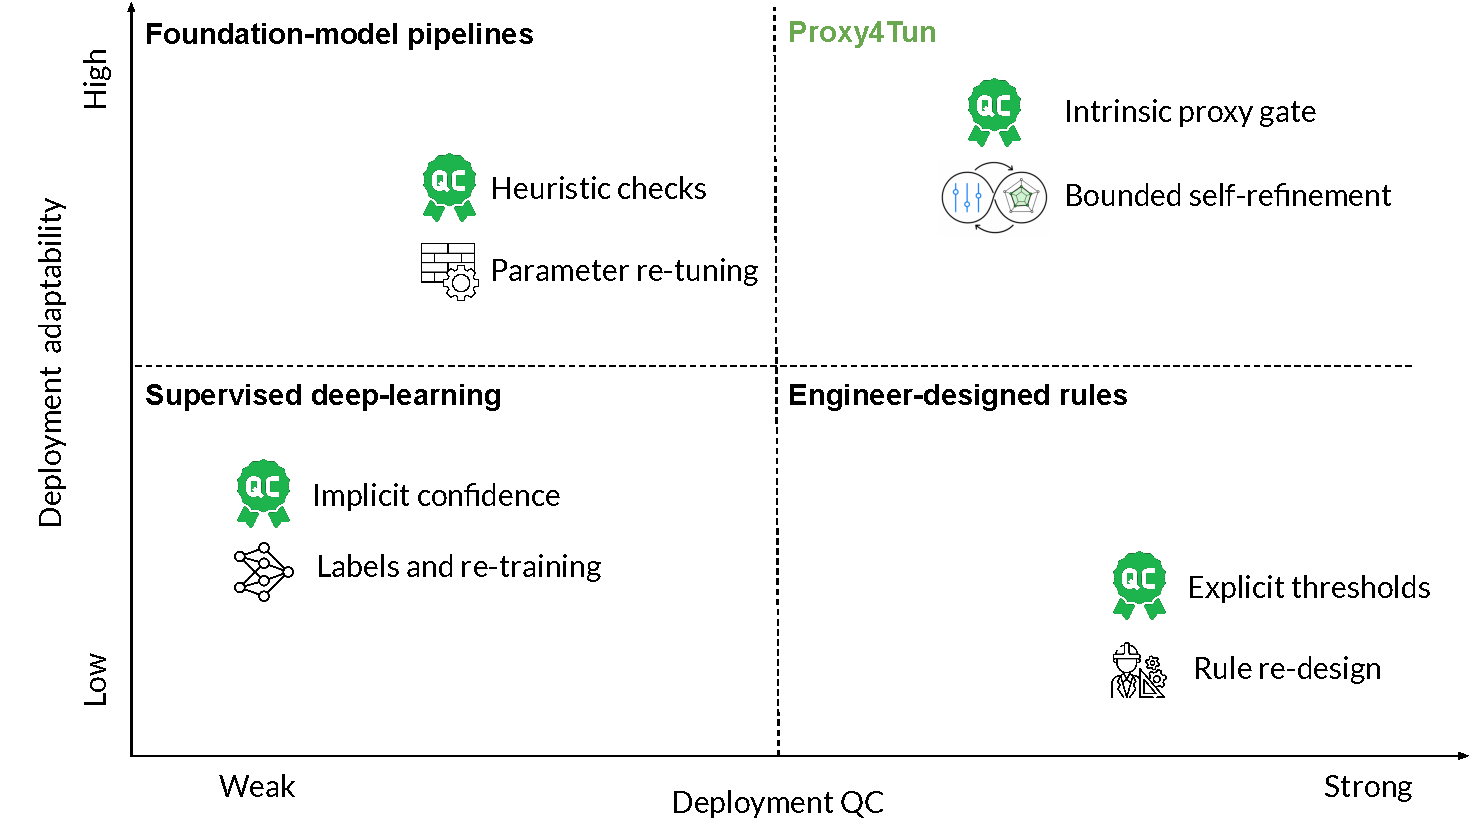
\includegraphics[width=0.9\textwidth]{figs/position.pdf}
\caption{Proxy4Tun's positioning: Conceptual positioning of segmentation paradigms by deployment adaptability and deployment QC strength. Engineer-designed rules provide explicit QC through predefined thresholds and checks but may require expert rule redesign when deployment conditions change. Supervised deep-learning methods adapt through labelled retraining but generally lack an explicit deployment-time accept/refine/reject gate, while foundation-model pipelines support Parameter-based adaptation but rely mainly on heuristic output checks. Proxy4Tun targets the high-adaptability, strong-QC region by combining bounded deployment-time self-refinement with an explicit intrinsic proxy gate.}
\label{fig:conceptual_positioning}
\end{figure*}

This study contributes a quality-estimation mechanism, not a complete deployment system: absolute segmentation quality remains bounded by the underlying SAM4Tun stage algorithms and the single anchor per family, and the reflective loop is evaluated as a five-subset PoC. Within that scope, the evaluation isolates what a frozen linear proxy over stage-observable metrics can and cannot see.

This paper makes the following contributions:
\begin{enumerate}
\item A deployment-label-free quality-estimation formulation for segmental tunnel-lining segmentation that couples a GT-free intrinsic proxy over evidence and coherence features with accept/refine/flag decisions on a unified pipeline spanning staggered, continuous, and complex linings.
\item A design-time calibration protocol in which space-filling BO exploration around one anchor per family (40 trials each, all six stages tunable) is distilled by leave-one-out feature ablation and a permutation control into a frozen five-feature pooled Ridge proxy.
\item Holdout evidence on 27 unseen subsets (54 scored runs): Spearman 0.848 and MAE 0.071 against GT mIoU, 27/27 anchor-versus-bad ranking, and perfect known-bad flagging, with ablation evidence that feature pruning drives cross-family transfer and that pooling preserves alarm recall relative to per-family refits.
\item A PoC reflective loop in which LLM-proposed bounded overlays are selected by proxy score, improving mIoU on four of five subsets ($+$0.040 to $+$0.353); the single failure is traced to a stage-1 geometry defect invisible to the pruned feature set, delimiting the proxy's scope and motivating stage-1 auditing as future work.
\end{enumerate}

The rest of this paper is organised as follows. Section~\ref{sec:related} reviews related work. Section~\ref{sec:methods} presents methodology, including the task definition, the Proxy4Tun architecture, the reflective agent, and the experimental design. Section~\ref{sec:results} reports results. Section~\ref{sec:discussion} discusses findings, positioning, and limitations. Section~\ref{sec:conclusions} concludes.

% ══════════════════════════════════════════════════════════════════════════
\section{Related work}\label{sec:related}
% ══════════════════════════════════════════════════════════════════════════

This study situates Proxy4Tun among (i)~tunnel and infrastructure point-cloud segmentation, (ii)~deployment-time quality control without labels, (iii)~Bayesian optimisation as design-time experience generation, and (iv)~reflective LLM agents for iterative refinement. The distinguishing requirement is \emph{deployment control}: accept, refine, or flag a multi-stage tunnel pipeline when GT is unavailable.

\subsection{Tunnel and infrastructure point-cloud segmentation}

Tunnel inspection surveys motivate automated extraction of lining components from terrestrial laser scanning (TLS) and photogrammetry~\cite{attard2018,montero2015,sjolander2023towards}. Geometric and feature-engineered pipelines fit centrelines, unroll surfaces, and apply density or curvature rules~\cite{weidner2024generalized,huang2021bim,wang2025automated}; their logic is auditable but brittle when diameter, joint pattern, or density change. Supervised deep models on point clouds---PointNet++~\cite{qi2017pointnet}, RandLA-Net~\cite{hu2020randla}, Mask3D~\cite{schult2023mask3d}, and top-down instance segmentation~\cite{kolodiazhnyi2024td3d}---together with tunnel-specific networks and reviews~\cite{duan2023high,su2024review,cha2024deep,wang2026serialformer,ye2026maintenance} improve adaptability when labels exist, yet labelled tunnel corpora remain scarce and retraining is costly for each new lining family. Seg2Tunnel provides a public segmental-lining benchmark~\cite{lin2024seg2tunnel}. Foundation-model pipelines project tunnels to panoramic depth maps and prompt SAM~\cite{kirillov2023sam,ye2024sam,ge2024cracksam}; SAM4Tun~\cite{ye2025sam4tun} achieves strong expert-tuned accuracy but exposes dozens of stage parameters that do not transfer off the reference. Proxy4Tun keeps that stage graph fixed and focuses on \emph{controlling} it at deployment rather than replacing the segmenter.

\subsection{Deployment-time quality control without labels}

When GT is absent, segmentation systems need secondary signals for reliability. Early work estimated segmentation error without labels~\cite{kohlberger2012segmentationError}; reverse classification accuracy and related QC scores similarly assess trustworthiness from model behaviour or image evidence~\cite{valindria2017rca,robinson2018segmentationQuality,fournel2021segmentationQC,cosarinsky2025inContextRCA}. Related work detects erroneous surface regions~\cite{zaman2023erroneousSurfaceRegions} or LiDAR perception failures~\cite{bogdoll2025lidarFailureDetection}, and uncertainty methods (dropout, ensembles, calibration) quantify predictive confidence~\cite{gal2016dropout,kendall2017uncertainties,lakshminarayanan2017deepEnsembles,guo2017calibration,vassilev2024uncertaintyInfrastructure}. These approaches rarely encode tunnel-specific failure modes---mirrored unrolls, fallback-heavy detections, or within-ring phase rotations---nor do they expose an engineer-auditable accept/refine/flag decision tied to pipeline stages. Proxy4Tun builds the control signal from \emph{intrinsic stage artifacts} of the tunnel pipeline itself, calibrated once against mIoU on a small design panel and frozen as a five-feature linear model whose coefficients an engineer can inspect.

\subsection{Bayesian optimisation for design-time experience}

Bayesian optimisation (BO) efficiently searches expensive black-box objectives with Gaussian-process surrogates and acquisition rules such as Expected Improvement~\cite{mockus1978bayesian,jones1998ego,rasmussen2006gpml,snoek2012practicalBO,shahriari2016reviewBO,frazier2018tutorialBO,garnett2023bayesianOptimization}. In Proxy4Tun, BO is \emph{not} the deployment optimiser, and the goal of exploration is not the optimum. The BO framework---bounded per-family search spaces around each anchor---is used as a design-time experience generator: scrambled-Sobol space-filling sampling of the search space populates a corpus of high-, medium-, and low-quality trials so that intrinsic features can be related to GT mIoU across the whole quality range, including deliberate failures. An acquisition-driven optimiser would concentrate samples near good configurations and starve the proxy of the degraded examples it must learn to flag. The surrogate machinery is then discarded; only the frozen Ridge proxy and alarm threshold travel to deployment. This differs from using BO online on each new tunnel, which would reintroduce labels or an unverified surrogate at runtime.

\subsection{Reflective and agentic LLM refinement}

Reasoning-oriented LLMs support multi-step diagnosis via chain-of-thought and related protocols~\cite{wei2023cot,kojima2023zeroshot,xiang2025metacot}. Self-refinement, reflection, and act-observe loops iterate on feedback without gradient updates~\cite{madaan2023selfrefine,shinn2023reflexion,yao2023react,ferraz2024llm}, and LLM agents have been applied to engineering and scientific workflows including chemical synthesis planning~\cite{bran2024chemcrow}, protein discovery~\cite{ghafarollahi2024protagents}, multi-agent software collaboration~\cite{qian2024chatdev,hong2024metagpt}, and manufacturing decision support~\cite{garcia2024manufacturing}. All of these loops presuppose a feedback signal; in most engineering pipelines no label-free critic exists. Proxy4Tun supplies that critic: in the PoC loop, an LLM agent prompted with the tunnel ontology inspects GT-free intrinsics and artifacts, proposes bounded multi-stage parameter overlays, and each round is scored by the frozen proxy, with the highest-scoring configuration retained. Unlike open-ended agent coding, the action space is the pipeline parameter schema; unlike one-shot LLM adaptation, reflection is closed-loop on live artifacts. The same frozen proxy could in principle serve as a reward signal for reinforcement-learning-based tuning, which we leave to future work.

% ══════════════════════════════════════════════════════════════════════════
\section{Methodology}\label{sec:methods}
% ══════════════════════════════════════════════════════════════════════════

Our methodology defines the deployment-label-free quality-control task for segmental tunnel-lining segmentation, summarises the fixed unified pipeline across lining families, and specifies the Proxy4Tun layer: design-time BO exploration that generates labelled experience, a GT-free intrinsic proxy calibrated on that experience, and a reflective agent that reads the proxy together with ontology-grounded context to propose bounded parameter updates. We then describe the dataset, feature-set ablation, holdout protocol, and metrics.

\subsection{Task definition}\label{sec:problem-def}

The upstream task is semantic segmentation of segmental tunnel linings from TLS point clouds. Given a raw point cloud of a tunnel section, the goal is to assign each point a structural label: background, key segment~(K), adjacent segments (B), and standard segments (A), with an additional A4 class for 7-segment complex tunnels. The unit of analysis is a tunnel subset spanning multiple rings selected from the Seg2Tunnel benchmark.

\begin{figure*}[t]
\centering
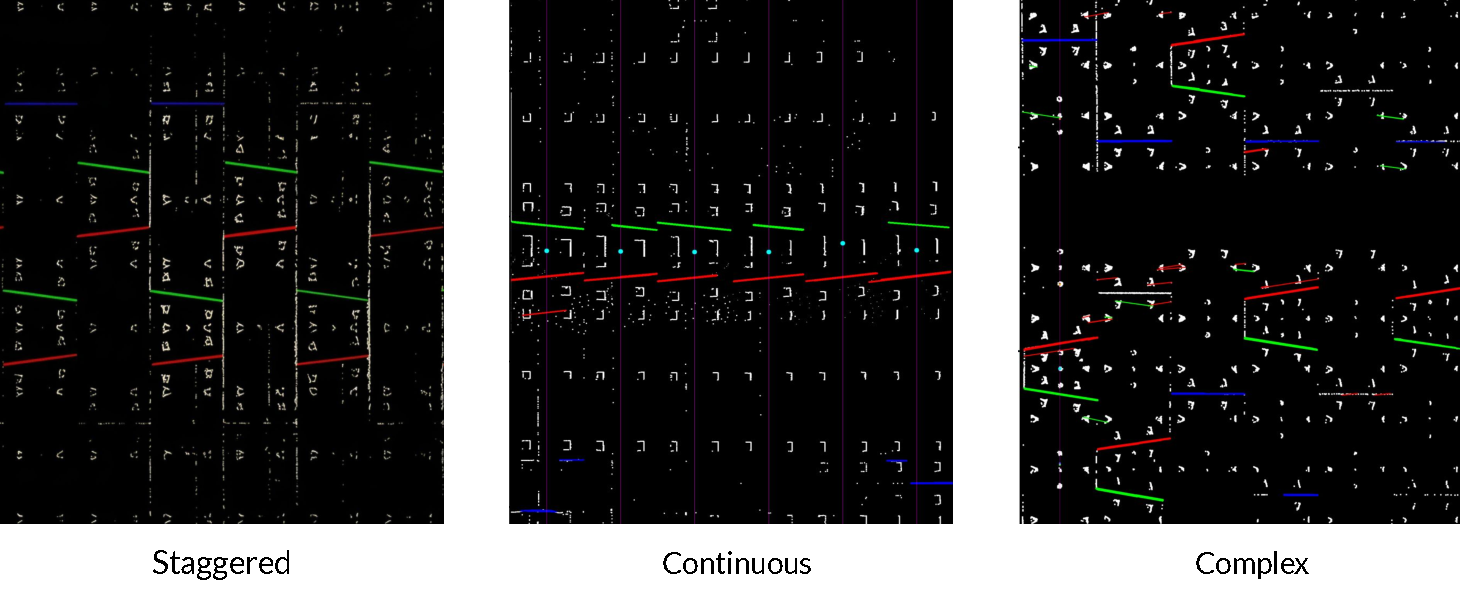
\includegraphics[width=0.9\textwidth]{figs/task.pdf}
\caption{Task definition: Proxy4Tun aims to provide a unified lightweight quality proxy across the three tunnel families (Staggered/Continuous/Complex) of the Seg2Tunnel dataset. At deployment, it predicts the direction of mIoU for a new tunnel processed by a parameterised pipeline, without ground truth, using only the declared family and the segments-per-ring count (6 or 7) as a consistency check.}
\label{fig:task}
\end{figure*}

A fixed expert configuration of the open-source SAM4Tun pipeline transfers poorly when lining layout, diameter, or scanning geometry depart from the tuning reference, and the pipeline provides no built-in signal indicating which runs have degraded. At deployment, GT labels are typically unavailable for either retuning or post-hoc quality control. Proxy4Tun addresses this gap: it does not alter the underlying stage algorithms, but learns a GT-free score that ranks candidate parameterisations and raises an alarm when a run is likely to be low quality (Fig.~\ref{fig:task}). GT mIoU is used only at design time for proxy calibration and for offline evaluation of the proxy itself.

\subsection{Proxy4Tun}\label{sec:method}

\begin{figure*}[t]
\centering
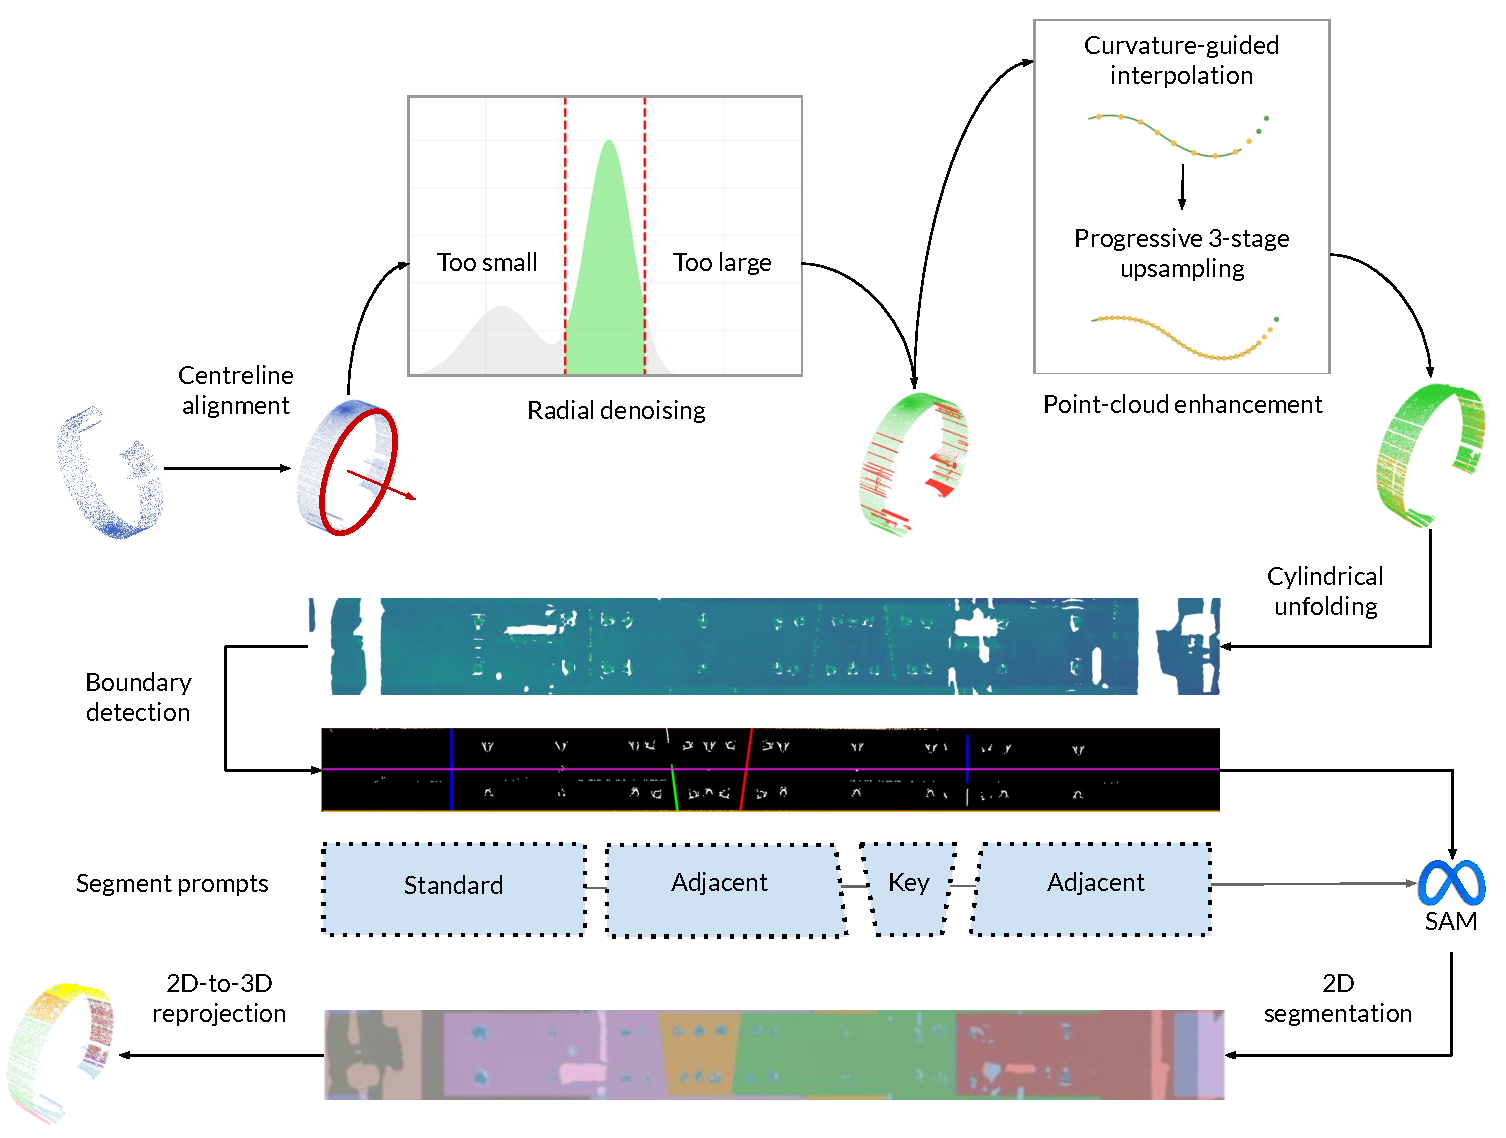
\includegraphics[width=0.98\textwidth]{figs/pipeline.pdf}
\caption{Segmentation pipeline: the pipeline is adapted and parameterised from SAM4Tun~\cite{ye2025sam4tun} for all tunnel families and is illustrated using successive representations of an example ring. The raw point cloud is first centreline-aligned and radially denoised by retaining points within the expected lining-radius range. The retained surface is then enhanced through curvature-guided interpolation and progressive three-stage upsampling before cylindrical unfolding into a two-dimensional depth map. Hough-transform-based boundary detection identifies candidate ring-joint lines, from which prompt templates for the key segment, adjacent segments, and standard segments are constructed and supplied to the Segment Anything Model (SAM). The resulting 2D segment masks are finally reprojected onto the original three-dimensional ring point cloud. (\textit{Note:} the tunable parameters and family-specific anchor profiles are listed in Table~\ref{tab:anchor-params}.)}
\label{fig:pipeline}
\end{figure*}

\begin{table*}[t]
\caption{Expert-tuned, family-specific anchor parameter profiles of the segmentation pipeline, provided by the first author of SAM4Tun.}\label{tab:anchor-params}
\begin{tabular*}{\textwidth}{@{\extracolsep{\fill}} l l p{0.30\textwidth} l @{}}
\toprule
Stage & Parameter & Description & Staggered / Continuous / Complex \\
\midrule
Unfolding & \texttt{diameter} & Cylindrical scale. & 5.5 / 5.9 / 7.5\,m \\
Unfolding & \texttt{slice\_spacing\_factor} & Slice spacing (ring width). & 1.2 / 1.2 / 1.8\,m \\
Unfolding & \texttt{polynomial\_degree} & Centreline fit degree. & 3 / 2 / 2 \\
Unfolding & \texttt{residual\_recentre} & Per-bin frame recentring. & off / on / on \\
\midrule
Denoising & \texttt{mask\_r\_low} & Inner radial gate. & 2.33 / 2.85 / 3.65\,m \\
Denoising & \texttt{mask\_r\_high} & Outer radial gate. & 2.78 / 3.0 / 3.9\,m \\
Denoising & \texttt{y\_step} & Angular bin width. & 0.4 / 0.5 / 0.1\,m \\
Denoising & \texttt{z\_step} & Radial histogram bin width. & 0.005 / 0.001 / 0.001\,m \\
Denoising & \texttt{grad\_threshold} & Outer-edge gradient threshold. & 0.15 / 0.2 / 0.2 \\
Denoising & \texttt{smoothing\_window\_size} & Cutoff-curve smoothing window. & 5 / 3 / 3 \\
Denoising & \texttt{smoothing\_offset} & Post-smoothing cutoff bias. & $-$0.002 / $-$0.003 / $-$0.005\,m \\
Denoising & \texttt{default\_cutoff\_z} & Fallback radial cutoff. & 2.75 / 2.85 / 3.65\,m \\
\midrule
Enhancing & \texttt{upsampling\_stage1} & Stage-1 upsampling spacing. & 0.06 / 0.08 / 0.09\,m \\
Enhancing & \texttt{upsampling\_stage2} & Stage-2 upsampling spacing. & 0.03 / 0.04 / 0.045\,m \\
Enhancing & \texttt{upsampling\_stage3} & Stage-3 upsampling spacing. & 0.015 / 0.02 / 0.0225\,m \\
Enhancing & \texttt{curvature\_threshold} & Panel--joint curvature threshold. & 0.005 / 0.0005 / 0.0005 \\
Enhancing & \texttt{depth\_threshold\_low} & Lower interpolation depth tolerance. & 0.005 / 0.01 / 0.0065\,m \\
Enhancing & \texttt{depth\_threshold\_high} & Upper interpolation depth tolerance. & 0.015 / 0.01 / 0.013\,m \\
Enhancing & \texttt{inter\_radius} & Interpolation neighbour radius. & 0.03 / 0.06 / 0.06\,m \\
Enhancing & \texttt{n\_segment\_start/end} & Interpolated ring-index window. & 0--5 / 2--8 / 5--14 \\
Enhancing & \texttt{ring\_spacing\_factor} & Nominal ring width. & 1.2 / 1.2 / 1.8\,m \\
\midrule
Detecting & \texttt{binary\_threshold} & Depth-map binarisation level. & 125 / 127 / 125 \\
Detecting & \texttt{hough\_thresh\_obliq} & Oblique joint-line vote threshold. & 65 / 30 / 35 \\
Detecting & \texttt{hough\_thresh\_horiz} & Horizontal joint-line vote threshold. & 65 / 30 / 35 \\
Detecting & \texttt{hough\_thresh\_vert} & Ring-boundary vote threshold. & 600 / 1500 / 5000 \\
Detecting & \texttt{minLineLength\_obliq} & Minimum oblique line length. & 100 / 40 / 80\,px \\
Detecting & \texttt{minLineLength\_horiz} & Minimum horizontal line length. & 100 / 50 / 80\,px \\
Detecting & \texttt{maxLineGap\_obliq} & Oblique line-merging gap limit. & 45 / 30 / 60\,px \\
Detecting & \texttt{maxLineGap\_horiz} & Horizontal line-merging gap limit. & 10 / 10 / 15\,px \\
Detecting & \texttt{angle\_range\_oblique} & Oblique-joint angle band. & $\pm$[6, 9] / $\pm$[4, 10] / $\pm$[5, 10]$^{\circ}$ \\
\midrule
Segmenting & \texttt{segment\_per\_ring} & Segments per lining ring. & 6 / 6 / 7 \\
Segmenting & \texttt{segment\_order} & Circumferential segment order. & \begin{tabular}[t]{@{}l@{}}K,B1,A1--A3,B2 /\\K,B2,A3--A1,B1 /\\K,B1,A1--A4,B2\end{tabular} \\
Segmenting & \texttt{segment\_width} & Nominal segment width. & 1200 / 1200 / 1800\,mm \\
Segmenting & \texttt{K\_height} & Key-segment arc height. & 1079.9 / 823.8 / 1227.0\,mm \\
Segmenting & \texttt{AB\_height} & Standard-segment arc height. & 3239.8 / 3346.8 / 3726.9\,mm \\
Segmenting & \texttt{angle} & Oblique K-joint inclination. & 7.52 / 6.12 / 9.8$^{\circ}$ \\
Segmenting & \texttt{processing.y\_bounds} & Valid panorama band. & 3800--13300 / 4500--14000 / 4200--13100\,px \\
\bottomrule
\end{tabular*}
\end{table*}

\subsubsection{Unified pipeline}\label{sec:pipeline}

Proxy4Tun builds on a single unified stage graph adapted from SAM4Tun~\cite{ye2025sam4tun} (Fig.~\ref{fig:pipeline}) that covers the three Seg2Tunnel lining families---staggered (T1/T2), continuous (T3), and complex interleaved (T4/T5)---via a family-mode switch rather than separate code paths. \emph{Unfolding} establishes a cylindrical coordinate system: cross-sections are fit by RANSAC ellipse estimation~\cite{fischler1981ransac}, ellipse centres are interpolated into a smooth centreline, and the lining surface is projected into a panoramic depth map in which each pixel stores radial distance to the centreline. Orientation conventions (circumferential handedness, ring-index sign) are treated as invariants: a mirrored unroll can look geometrically clean while mapping every asymmetric class to its circumferential mirror, collapsing mIoU without an obvious cosmetic failure. \emph{Denoising} removes non-structural artefacts by grid-based radial-density filtering inspired by the DBSCAN clustering principle~\cite{ester1996dbscan}, constrained by radial masks $(R_\mathrm{low}, R_\mathrm{high})$; the retained-point ratio and residual empty-pixel structure of the depth map become primary evidence signals for the proxy. \emph{Enhancing} restores geometric continuity before detection through curvature-guided interpolation and progressive upsampling, preserving joint boundaries while densifying smooth panels. \emph{Detection and segmentation} recover joint lines with orientation-specific Hough thresholds~\cite{duda1972hough}, assemble template prompts under the family layout grammar, and invoke SAM~\cite{kirillov2023sam}; masks are reprojected to per-point 3D labels. Detection regularity and SAM layout statistics form the coherence half of the proxy feature set.

The pipeline exposes dozens of tunable parameters across geometry, filtering, interpolation, detection thresholds, and SAM crop settings (Table~\ref{tab:anchor-params}). Family anchors provide expert-tuned warm-start configurations; exploration perturbs a bounded overlay spanning all six stages, while the orientation flags remain pinned to the canonical frame. The stage algorithms remain fixed across all experimental conditions; only parameter values change. A staged ontology of artifacts, quality metrics, failure modes, and remediation actions supplies the diagnostic vocabulary from which the intrinsic feature blocks below are distilled.

\subsubsection{Intrinsic feature blocks}\label{sec:features}

Every completed run yields a vector of GT-free intrinsic metrics computed from stage artifacts. We organise the ten candidate metrics into two complementary groups aligned with the ontology's failure taxonomy (Table~\ref{tab:candidate-features}):

\begin{itemize}
\item \textbf{Evidence}---input and artifact quality across the projection stages: depth-map completeness (\texttt{depth\_nan\_ratio}), denoising retention (\texttt{denoise\_retained\_ratio}), and a stage-1 geometry audit pair (centreline recentring residual \texttt{unfold\_residual} and axis-orientation agreement \texttt{orient\_agreement}).
\item \textbf{Coherence}---structural plausibility of the detection and segmentation result: segment-mask fill rate, class-balance divergence from the equal-mass prior, the K-row detection residual and gate indicator, within-row anchor scatter, and cross-ring phase incoherence.
\end{itemize}

\begin{table*}[t]
\caption{The ten candidate features of the combined proxy P(e+c). Evidence
features audit input/artifact quality (stages 1--3); coherence features audit
the structural plausibility of the detection and segmentation result
(stages 4--5). All are computed from intermediate pipeline artifacts without
ground truth. The last column gives the standardised ridge weight for the five
features retained in the deployed lean model; pruned features are marked
``--''.}\label{tab:candidate-features}
\begin{tabular*}{\textwidth}{@{\extracolsep{\fill}} l l p{0.42\textwidth} c c @{}}
\toprule
Group & Feature & Meaning & Stage & Lean weight \\
\midrule
Evidence & \texttt{depth\_nan\_ratio} & Fraction of empty (white) pixels on the unfolded depth map. & 1--3 & $-$0.17 \\
Evidence & \texttt{denoise\_retained\_ratio} & Fraction of the point cloud surviving the radial denoising mask; high retention indicates under-filtering. & 2 & $-$0.39 \\
Evidence & \texttt{unfold\_residual} & Centreline recentring residual, $\log(1{+}\,\mathrm{cm})$ (stage-1 geometry audit). & 1 & -- \\
Evidence & \texttt{orient\_agreement} & Agreement $\lvert\mathrm{corr}(h, \text{PCA tunnel axis})\rvert$ between the unfolded axis and the point-cloud principal axis. & 1 & -- \\
\midrule
Coherence & \texttt{sam\_fill\_rate} & Fraction of points assigned a non-background segment label. & 5 & $+$0.47 \\
Coherence & \texttt{sam\_ontology\_divergence} & Total-variation distance between the predicted class-mass distribution and the equal-mass prior over segment classes. & 5 & -- \\
Coherence & \texttt{det\_row\_residual\_px} & Distance of detected K-row anchors from the design row pattern, $\log(1{+}\,\mathrm{px})$; meaningful only when gated. & 4 & $-$0.11 \\
Coherence & \texttt{det\_row\_gated} & Indicator that the K-row verification gate produced evidence for this run. & 4 & $+$0.13 \\
Coherence & \texttt{det\_row\_y\_std} & Within-row vertical scatter of K-row anchor points. & 4 & -- \\
Coherence & \texttt{phase\_incoherence\_deg} & Cross-ring circular distance of block-label ``clock faces''; detects per-ring label rotation. & 5 & -- \\
\bottomrule
\end{tabular*}
\end{table*}

Coherence features catch form and regularity failures; evidence features catch hollow or under-filtered runs that can still look locally regular. The deployed proxy does not use all ten candidates: leave-one-out feature ablation (Section~\ref{sec:comparators}) prunes the set to the five-feature \emph{lean} model whose standardised weights appear in Table~\ref{tab:candidate-features}. The phase-incoherence feature additionally powers an auxiliary alarm on regular linings (Section~\ref{sec:phase-alarm}).

\subsubsection{Bayesian-exploration experience generation}\label{sec:bo-experience}

\begin{figure*}[t]
\centering
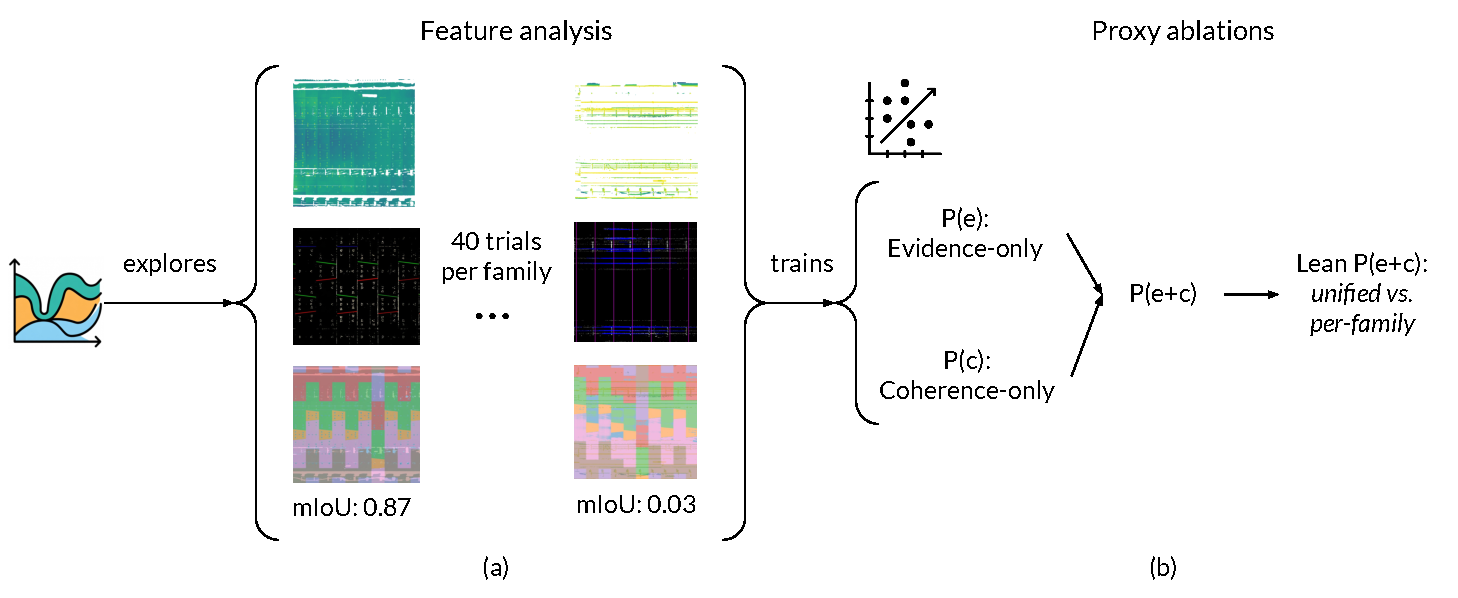
\includegraphics[width=1\textwidth]{figs/b-p.pdf}
\caption{Proxy ablations: (a)~Bayesian exploration of the parameter space around each family anchor generates 40 labelled trials per family (120 in total), spanning healthy (mIoU~0.87) to degraded (mIoU~0.03) configurations; each trial retains its intermediate artifacts (e.g. depth maps, detected lines, segment masks) and the corresponding feature value changes. (b)~The trials calibrate the mIoU proxy, ablated over feature sets: evidence-only $P(e)$ (3D-to-2D projection quality), coherence-only $P(c)$ (segmentation-structure consistency), and combined $P(e{+}c)$. From these, the leave-one-out-pruned, lean $P(e{+}c)$ is compared in unified and per-family forms. Ground-truth labels are used only during this calibration stage.}
\label{fig:b-p}
\end{figure*}

Design-time exploration reuses the BO technical framework---bounded per-family search spaces $\Theta_f$ around each anchor configuration $P^{*}_f$---but its goal is \emph{coverage} of the quality range, not the optimum (Fig.~\ref{fig:b-p}a). Scrambled-Sobol quasi-random sampling of $\Theta_f$ generates candidate overlays spanning all six pipeline stages (including stage-1 centreline knobs); each candidate is materialised over the anchor parameters and run through the full pipeline, recording the GT mIoU $y_i$ and the intrinsic feature vector $\mathbf{x}_i$ (Algorithm~\ref{alg:bo_exploration}). Space-filling sampling is deliberate: an acquisition-driven optimiser would concentrate trials near good configurations and starve the proxy of the degraded examples it must learn to flag. Failed or feature-incomplete runs are excluded and topped up, yielding exactly 40 valid trials per family (120 in total) that span healthy (mIoU~$\approx 0.87$) to collapsed (mIoU~$\approx 0.03$) configurations. Search-space bounds derive from the anchor values with modest padding and are truncated where the pipeline fails structurally rather than gracefully. From each family we additionally freeze one \emph{known-bad} overlay (a historically low-mIoU trial far below the sibling-anchor floor) for holdout stress testing.

\begin{algorithm}[ht]
\caption{Space-filling Exploration of the Full-Pipeline Parameter Space (BO framework)}\label{alg:bo_exploration}
\begin{algorithmic}[1]
\Require Family anchor configuration $P^{*}_{f}$ (expert-tuned reference parameters)
\Require Bounded search space $\Theta_f$ over all six stages with bounds $B$
\Require Target trial count $N$ per family
\Ensure Labelled trial set $\mathcal{T}_f = \{(\theta_i, \mathbf{x}_i, y_i)\}_{i=1}^{N}$ spanning healthy to degraded runs
\State \textbf{Phase 1: Space-filling candidate generation}
\State $U \gets \text{SobolSequence}(|\Theta_f|, N)$ \Comment{Scrambled quasi-random points in the unit cube}
\State $\{\theta_i\} \gets \text{DecodeToBounds}(U, \Theta_f, P^{*}_{f})$ \Comment{Bounded overlays on the anchor parameters}
\State \textbf{Phase 2: Full-pipeline trial execution}
\For{each candidate $\theta_i$}
    \State $P_i \gets \text{Materialise}(P^{*}_{f}, \theta_i)$ \Comment{Anchor parameters with overlay applied}
    \State $r_i \gets \text{RunPipeline}(P_i, \text{stages } 1\text{--}6)$ \Comment{Re-run per trial; no frozen checkpoint}
    \State $y_i \gets \text{Evaluate}(r_i)$ \Comment{GT mIoU; labels used only here}
    \State $\mathbf{x}_i \gets \text{ExtractFeatures}(r_i, P_i)$ \Comment{GT-free Evidence--Coherence vector}
\EndFor
\State \textbf{Phase 3: Quality gate and top-up}
\State $\mathcal{T}_f \gets \{(\theta_i, \mathbf{x}_i, y_i) : \text{status ok} \wedge \mathbf{x}_i \text{ complete}\}$
\While{$|\mathcal{T}_f| < N$}
    \State Draw further Sobol candidates and repeat Phase 2 \Comment{Failed runs are excluded, not averaged in}
\EndWhile
\State \Return $\mathcal{T}_f$ \Comment{Coverage of the quality range, not an optimum, is the goal}
\end{algorithmic}
\end{algorithm}

\subsubsection{Pooled lean Ridge proxy}\label{sec:ridge-proxy}

Let $\mathbf{x}\in\mathbb{R}^{d}$ denote the intrinsic feature vector of a completed run and $y$ its GT mIoU. Features are standardised using the training mean $\boldsymbol{\mu}$ and scale $\boldsymbol{\sigma}$, and a single $\ell_2$-regularised linear regressor is fitted by cross-validated RidgeCV on the pooled 120 trials from all three family anchors:
\begin{equation}
\widehat{\text{mIoU}}(\mathbf{x})
= \mathbf{w}^{\top}\!\left(\frac{\mathbf{x}-\boldsymbol{\mu}}{\boldsymbol{\sigma}}\right) + b,
\label{eq:ridge-proxy}
\end{equation}
with regularisation strength selected on the training folds. Standardisation makes the coefficient magnitudes directly comparable, so the frozen weights (Table~\ref{tab:candidate-features}) double as a sensitivity record (Section~\ref{sec:sensitivity}). The lean feature set is selected by leave-one-out ablation with leave-one-family-out cross-validation, and a permutation control (refitting on label-shuffled trials, 20 repeats) verifies that the learned relationship exceeds Ridge capacity alone. Pooling is a deliberate design choice validated in the ablation: per-family refits of the same lean features are retained as a comparator (Section~\ref{sec:proxy-ablation-results}), but the pooled model triples the effective training data per family and preserves alarm recall.

An alarm threshold $\tau$ is calibrated on training predictions so that low proxy scores flag likely low-mIoU runs. At deployment, the frozen $(\widehat{\text{mIoU}},\tau)$ pair scores candidates without labels, requiring only the family declaration (which selects the class-count prior and gate applicability during feature extraction) and the segments-per-ring count. Figure~\ref{fig:proxy-training} shows the training fit; holdout fidelity is evaluated in Section~\ref{sec:main-results}. Algorithm~\ref{alg:bo_exploration} summarises design-time exploration; Algorithm~\ref{alg:proxy} summarises calibration and deployment scoring.

\begin{figure}[t]
\centering
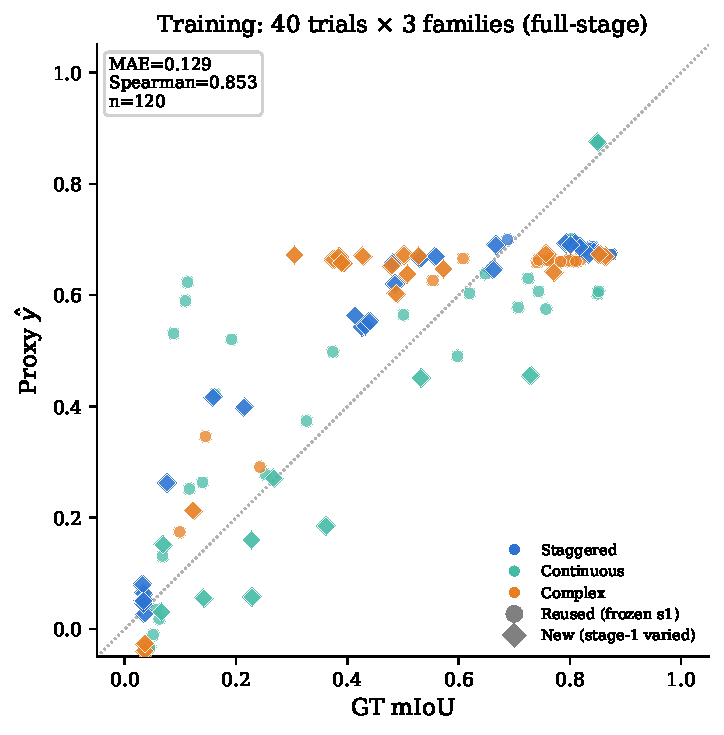
\includegraphics[width=0.75\columnwidth]{figs/proxy_training_fullstage.pdf}
\caption{Proxy training on the Bayesian-exploration corpus: proxy $\widehat{\text{mIoU}}$ versus GT mIoU on the 120 trials (40 each from the staggered, continuous, and complex anchors; identity dashed). Train MAE~$=0.129$, Spearman~$\rho=0.853$.}
\label{fig:proxy-training}
\end{figure}

\begin{algorithm}[ht]
\caption{Proxy Calibration and GT-free Deployment Scoring}\label{alg:proxy}
\begin{algorithmic}[1]
\Require Pooled trial sets $\mathcal{T} = \bigcup_{f} \mathcal{T}_f$ (Algorithm~\ref{alg:bo_exploration}, $N$ per family)
\Require Candidate feature set $F$ (Evidence $\cup$ Coherence)
\Ensure Frozen proxy $g$; deployment-time estimate $\widehat{\text{mIoU}}(r)$
\State \textbf{Phase 1: Standardisation}
\State $(\boldsymbol{\mu}, \boldsymbol{\sigma}) \gets \text{FitScaler}(\{\mathbf{x}_i\})$; \quad $\tilde{\mathbf{x}}_i \gets (\mathbf{x}_i - \boldsymbol{\mu}) / \boldsymbol{\sigma}$
\State \textbf{Phase 2: Ridge regression}
\State $g \gets \text{RidgeCV}(\{(\tilde{\mathbf{x}}_i, y_i)\})$ \Comment{Regularisation $\alpha$ selected by cross-validation}
\State \textbf{Phase 3: Feature ablation}
\For{each variant $V \in \{\text{Evidence}, \text{Coherence}, F\} \cup \{F \setminus \{v\} : v \in F\}$}
    \State Fit $g_V$; record train MAE/Spearman and leave-one-case-out error \Comment{Held-out anchor per fold}
\EndFor
\State $F_{\text{lean}} \gets \text{SelectLean}(\{g_V\})$ \Comment{Smallest set preserving full-set correlation}
\State \textbf{Phase 4: Permutation control}
\State Refit on label-shuffled $\{y_i\}$; require $\rho_{\text{real}} \gg \rho_{\text{perm}}$ \Comment{Reject feature--label leakage}
\State \textbf{Phase 5: Freeze}
\State Store $(\boldsymbol{\mu}, \boldsymbol{\sigma}, \mathbf{w}, b, \alpha, F_{\text{lean}})$ and alarm threshold $\tau$ \Comment{No further label access}
\State \textbf{Deployment (GT-free):} given run $r$ with declared family $f$ and segment count $C$
\State $\mathbf{x}(r) \gets \text{ExtractFeatures}(r)$ \Comment{From intermediate artifacts only}
\State $\widehat{\text{mIoU}}(r) \gets \mathbf{w}^{\top} \big( (\mathbf{x}(r) - \boldsymbol{\mu}) / \boldsymbol{\sigma} \big) + b$
\If{$\widehat{\text{mIoU}}(r) < \tau$} raise low-quality alarm \EndIf
\State \Return $\widehat{\text{mIoU}}(r)$
\end{algorithmic}
\end{algorithm}

\subsubsection{Phase-coherence alarm}\label{sec:phase-alarm}

Intrinsic regression can miss a specific failure mode: within-ring \emph{block-label rotation}, where segment form is coherent and evidence ratios look healthy, yet the circumferential phase of labels is wrong relative to neighbouring rings. For staggered and continuous families we therefore add a GT-free phase check: each ring's predicted block clock is compared to its nearest peer rings; large clock-face disagreement raises a phase alarm. The deployment alarm is the logical OR of the proxy threshold and the phase check. Complex (T4/T5) rings lack a stable repeating phase prior under interleaved keys, so the phase check is marked inapplicable there.

\subsection{Reflective agent design}\label{sec:agent-design}

\begin{figure*}[t]
\centering
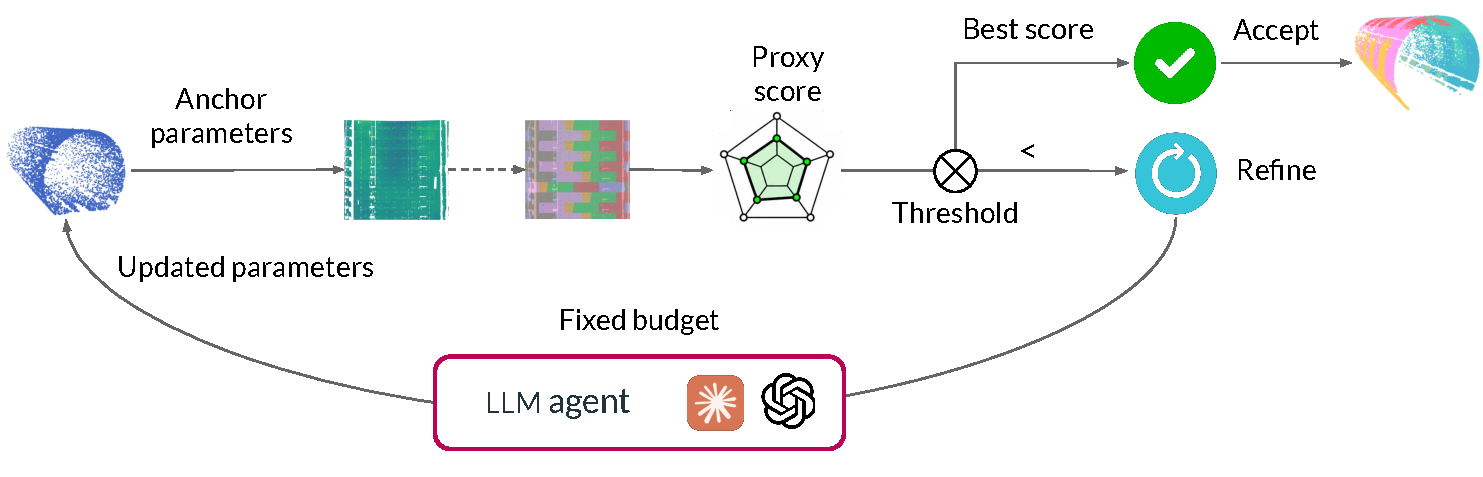
\includegraphics[width=0.9\textwidth]{figs/verification.pdf}
\caption{Proof-of-concept proxy verification: each held-out subset is first processed by the parameterised pipeline using the anchor parameters of its tunnel family and scored by the learned proxy. Subsets scoring at or above the threshold ($\tau = 0.7$) are accepted directly; otherwise, a large language model (LLM) agent (Fable~5 or GPT-5.6, prompted with the tunnel ontology) inspects the result and proposes updated parameters. The loop repeats within a fixed refinement budget, after which the highest-scoring configuration is retained. Accepted results are subsequently evaluated against ground truth (mIoU). This PoC is intended to demonstrate the proxy's potential as a self-refinement signal for reflective LLM agents or reinforcement learning (RL).}
\label{fig:verification}
\end{figure*}

The proxy ranks and alarms; it does not by itself choose which parameters to change. Proxy4Tun therefore couples the frozen proxy to a \emph{reflective agent} layer that proposes bounded parameter overlays without GT (Fig.~\ref{fig:verification}). The agent's context comprises the family anchor priors and warm-start parameters, the live post-stage artifacts and intrinsic metrics of the current candidate, the staged ontology (diagnostic rules, failure modes, remediation actions, and inter-stage dependencies), and the frozen proxy score and alarms injected as first-class signals. The agent is instructed to treat the proxy as a \emph{directional} improvement signal: round-to-round score changes and corroborating artifacts take precedence over the raw value, and a proxy increase driven only by evidence features while coherence degrades is treated as suspect.

Reflection follows a five-step protocol (Algorithm~\ref{alg:reflective_adaptation}) executed once per round within a fixed budget:
\begin{enumerate}
    \item \emph{Referencing:} Compare the current tunnel's priors and warm-start parameters against the family anchor; note the family mode and which stage-1 orientation knobs are pinned.
    \item \emph{Diagnostic inspection:} Evaluate ontology diagnostic rules against the live metrics and artifacts; emit matched failure modes. Check the phase alarm before attributing failure to detection or SAM.
    \item \emph{Upstream causal check:} Consult inter-stage dependencies; if a matched failure is likely caused upstream, defer to the upstream stage rather than retuning local parameters in the current round.
    \item \emph{Bounded adaptation:} Propose remediation actions with concrete parameter deltas inside the documented bounds, respecting the causal priority orientation $\rightarrow$ centreline $\rightarrow$ radial band $\rightarrow$ detection $\rightarrow$ SAM.
    \item \emph{Proxy-guided validation and JSON output:} Self-check logical constraints (e.g.\ $R_\mathrm{low}<R_\mathrm{high}$); reject proposals that flip pinned orientation knobs; emit a schema-conformant JSON overlay. After execution, accept the round only if the proxy improves (or the alarm clears) without coherence collapse; otherwise revert.
\end{enumerate}

Stage scripts and evaluation code are identical across rounds---only the parameter overlay changes---and every proposal is logged with a textual rationale for engineer review or override. Reflection is closed-loop on live artifacts: each round observes the pipeline outputs of the previous proposal, scores them with the GT-free proxy, and may defer changes when an upstream failure is the likely cause. To keep attribution clean, stage-1 artifacts are frozen when comparing stage-2--5 overlays; unfolding overlays, when needed, trigger a full rerun.

\begin{algorithm}[ht]
\caption{Proxy-guided reflective parameter adaptation}\label{alg:reflective_adaptation}
\begin{algorithmic}[1]
\Require Subset; family $f$; anchor priors and warm-start $P_{\mathrm{ref}}$; ontology with bounds $B$ and dependencies $D$; frozen proxy $(\widehat{\text{mIoU}},\tau)$; budget $R$
\Ensure Accepted overlay $P^\star$ (or flagged baseline)
\State Run unified pipeline with warm-start; compute $\mathbf{x}$, $\hat{y}\gets\widehat{\text{mIoU}}(\mathbf{x})$, alarms
\State $P^\star\gets P_{\mathrm{ref}}$; $\hat{y}^\star\gets\hat{y}$
\For{$r=1,\ldots,R$}
    \State \textbf{Steps 1--2:} Assemble live context; match diagnostic rules; list failure modes
    \State \textbf{Step 3:} If any failure has likely upstream cause in $D$, set active stage $\leftarrow$ upstream; else local stage
    \State \textbf{Step 4:} Propose $P_{\mathrm{proposed}}$ within bounds $B$ for the active stage
    \State \textbf{Step 5:} Validate constraints; reject pinned-orientation flips; format JSON overlay
    \State Execute pipeline (freeze stage~1 when overlay excludes unfolding); recompute $\mathbf{x}',\hat{y}',\mathrm{alarms}'$
    \If{$\hat{y}'>\hat{y}^\star$ \textbf{and} coherence not degraded}
        \State $P^\star\gets P_{\mathrm{proposed}}$; $\hat{y}^\star\gets\hat{y}'$
    \Else
        \State Revert overlay; continue or stop if no safe improvement remains
    \EndIf
    \If{$\hat{y}^\star>\tau$ \textbf{and not} phase-alarmed}
        \State \textbf{break} \Comment{Accept}
    \EndIf
\EndFor
\State \Return $P^\star$ (flag for review if still alarmed)
\end{algorithmic}
\end{algorithm}

\subsection{Experimental setup}\label{sec:exp-setup}

\subsubsection{Dataset}\label{sec:dataset}

We use Seg2Tunnel~\cite{lin2024seg2tunnel} multi-ring subsets spanning the three lining families (Table~\ref{tab:dataset}). Training experience comprises one labelled anchor case per family (2-1 staggered, 3-1 continuous, 5-1 complex), each explored with 40 space-filling trials over the bounded family search space (all six stages tunable), yielding 120 trials in total. Holdout evaluation uses 27 unseen subsets (9 per family, drawn from tunnels T1--T5), each scored under both the sibling-anchor configuration and the family's frozen known-bad overlay (54 scored runs). GT labels are used for offline mIoU and for proxy calibration only; they are never provided to the proxy at scoring time.

\begin{table*}[t]
\caption{Dataset and proxy-evaluation panel.}\label{tab:dataset}
\begin{tabular*}{\textwidth}{@{\extracolsep{\fill}} l l l l @{}}
\toprule
 & \multicolumn{2}{c}{Regular (T1, T2, T3)} & Complex (T4, T5) \\
\cmidrule(lr){2-3}\cmidrule(l){4-4}
Property & Staggered (T1, T2) & Continuous (T3) & \\
\midrule
Inner diameter & 5.5\,m & 5.9\,m & 7.5\,m \\
Ring length & 1.2\,m & 1.2\,m & 1.8\,m \\
Segments/ring & 6 & 6 & 7 \\
Joint type & Staggered & Continuous & Complex interleaved \\
Key-segment position & Ring-to-ring repeating pattern & Fixed ring-wise order & No repeating pattern \\
Scanning & Single-station & Multi-station & Single-station, offset \\
Eval.\ schema & 6-class & 6-class & 7-class \\
BO training anchor & 2-1 & 3-1 & 5-1 \\
Holdout subsets & 1-1{\ldots}1-5, 2-2{\ldots}2-5 & 3-2{\ldots}3-10 & 4-1{\ldots}4-5, 5-2{\ldots}5-5 \\
\bottomrule
\end{tabular*}
\end{table*}

\subsubsection{Experimental design}\label{sec:comparators}

The study follows a feature-set ablation that isolates each proxy component while holding the unified pipeline and holdout grid fixed (Table~\ref{tab:proxy-ablation}). All fits reuse the frozen 120-trial training table and the 54 holdout run manifests; no new pipeline runs are introduced during ablation. Conditions vary (i)~the feature set (evidence-only, coherence-only, combined, and the leave-one-out-pruned lean set) and (ii)~the model structure (one pooled Ridge on all 120 trials vs.\ one Ridge per family on its 40 trials, with identical lean features).

\begin{table}[ht]
\caption{Proxy ablation conditions.}\label{tab:proxy-ablation}
\begin{tabular*}{\tblwidth}{@{} c >{\raggedright\arraybackslash}p{2.3cm} >{\raggedright\arraybackslash}p{4.2cm} @{}}
\toprule
Level & Ablation & Condition \\
\midrule
1 & P(e) & Evidence only: 3D-to-2D projection quality \\
2 & P(c) & Coherence only: segmentation-structure consistency \\
3 & P(e+c) & Combined evidence + coherence \\
4 & Lean P(e+c) & Leave-one-out-pruned P(e+c), one model on all 120 trials \\
4a & \begin{tabular}[t]{@{}l@{}}Lean P(e+c) \\ per-family\end{tabular} & Same pruned features, one model per family (40 trials each) \\
\bottomrule
\end{tabular*}
\end{table}

As a capacity control, we permute mIoU labels within each family, refit the lean model, and repeat (20 shuffles). A large gap between real and permuted error indicates that the fit exploits genuine feature--mIoU structure rather than Ridge capacity alone. Train-parity and holdout gates on representative subsets verify that the unified pipeline reproduces the experience-generating anchors before proxy metrics are interpreted.

The PoC self-refinement loop (Section~\ref{sec:agent-design}) is run on five held-out subsets with the configuration of Table~\ref{tab:poc-config}: an LLM agent proposes bounded multi-stage overlays, each round is re-scored by the frozen proxy, and the best-of-three rounds by proxy score is retained. Pipeline execution used a single NVIDIA RTX~5060 GPU; all proposed overlays and rationales were logged for post-hoc review.

\begin{table}[ht]
\caption{PoC agent configuration.}\label{tab:poc-config}
\begin{tabular*}{\tblwidth}{@{} l l @{}}
\toprule
Setting & Value \\
\midrule
Models & Fable 5, GPT 5.6 \\
Interface & Cursor (v2) agent harness \\
Context provided & Tunnel ontology, intrinsics, artifacts \\
Refinement budget & 3 rounds per subset \\
Acceptance threshold & Proxy score $\tau = 0.7$ \\
Output format & JSON parameter overlay per round \\
Failure handling & Failed rounds discarded \\
Selection rule & Best proxy score across rounds \\
\bottomrule
\end{tabular*}
\end{table}

\subsubsection{Evaluation metrics}\label{sec:metrics}

Segmentation quality for offline analysis is measured by mean Intersection-over-Union (mIoU). For class $c$,
\begin{equation}
\text{IoU}_c = \frac{\text{TP}_c}{\text{TP}_c + \text{FP}_c + \text{FN}_c}, \qquad
\text{mIoU} = \frac{1}{C} \sum_{c=1}^{C} \text{IoU}_c,
\end{equation}
where $C$ is the number of segmental segments (classes) within one ring ($C=6$ for regular tunnels; $C=7$ for complex tunnels).

For the proxy itself, segmentation metrics are insufficient: the proxy is a
regressor whose output must track, rather than equal, the true score. We
therefore evaluate proxy fidelity with four complementary metrics. Mean
absolute error (MAE) between predicted and ground-truth mIoU measures
calibration,
\begin{equation}
\text{MAE} = \frac{1}{n}\sum_{i=1}^{n}\left|\widehat{\text{mIoU}}_i - \text{mIoU}_i\right|,
\end{equation}
while Spearman rank correlation $\rho$ measures whether the proxy orders runs
correctly, which is the property exploited when the proxy acts as a selection
signal. Because the deployed proxy also serves as a low-quality alarm, we
report precision and recall of the alarm at threshold $\tau$ against
ground-truth low-mIoU runs. Generalisation across tunnel families is assessed
by leave-one-family-out cross-validation, and a permutation control (refitting
on label-shuffled trials) verifies that the learned relationship exceeds
chance. Ground truth is used in these evaluations only; the proxy never
accesses labels at deployment.

For proxy fidelity we report bootstrap 95\% CIs (resampling held-out subsets)
for the Spearman correlation between predicted and ground-truth mIoU, and a
permutation control in which the proxy is refit on label-shuffled trials
(20 permutations); the real model's error must fall outside the permuted
distribution. For the unified versus per-family comparison we use a Wilcoxon
signed-rank test on paired per-subset differences ($n=54$). The
self-refinement loop is a proof of concept over five subsets and is reported
per case without formal significance testing.

\subsubsection{Sensitivity analysis}\label{sec:sensitivity-method}
We assess the robustness of the frozen proxy along two axes.
(i)~\emph{Feature ablation}: each candidate feature is removed in turn and the
model refit; the change in held-out rank correlation identifies load-bearing
versus prunable features and yields the lean set.
(ii)~\emph{Coefficient influence}: because all features are standardised
before the ridge fit, coefficient magnitudes are directly comparable and
quantify each feature's marginal influence on the predicted mIoU.

% ══════════════════════════════════════════════════════════════════════════
\section{Results}\label{sec:results}
% ══════════════════════════════════════════════════════════════════════════

We report (i)~overall proxy performance: calibration on the exploration trials and fidelity, ranking, and alarm behaviour on the held-out subsets; (ii)~feature-set and structure ablations with a permutation control; (iii)~a proof-of-concept self-refinement loop driven by the frozen proxy; and (iv)~parameter sensitivity of the frozen model. GT mIoU is used only offline.

\subsection{Overall performance}\label{sec:main-results}

\begin{figure*}[t]
\centering
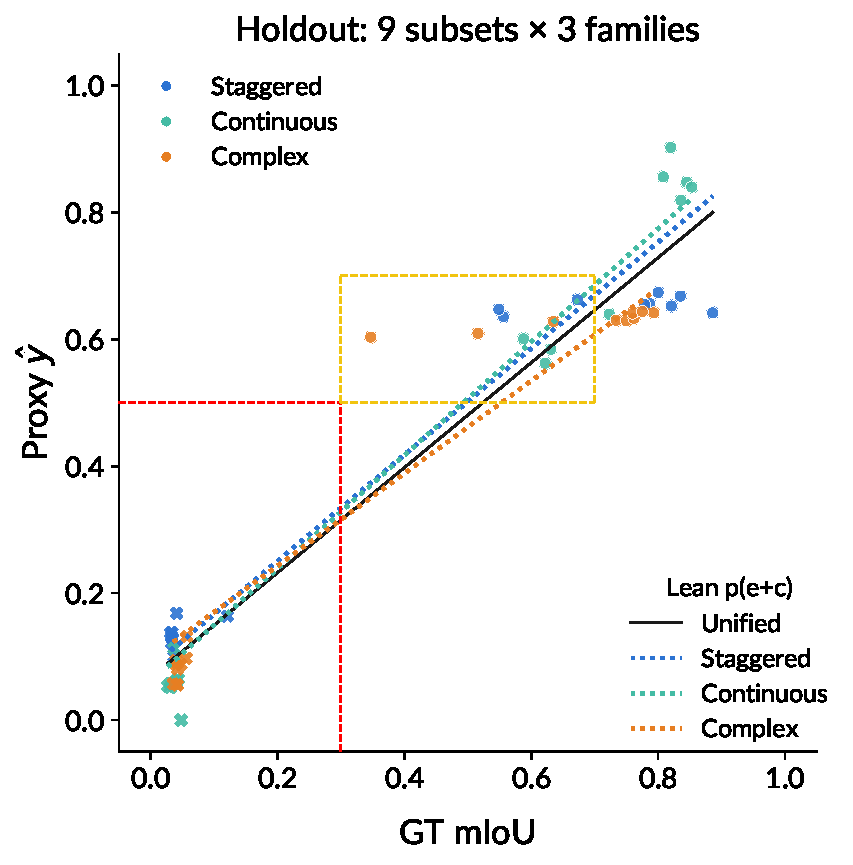
\includegraphics[width=0.85\textwidth]{figs/proxy_holdout_fullstage.pdf}
\caption{Proxy prediction versus ground-truth mIoU on the 27 held-out subsets
(54 scored runs: sibling-anchor and known-bad configuration per subset). Each
point is one pipeline run scored by the frozen lean proxy; the dashed line
marks the alarm threshold $\tau = 0.495$. Runs below the threshold are flagged
as low quality. Colours indicate lining family.}
\label{fig:holdout-scatter}
\end{figure*}

Before assessing the proxy on held-out tunnels, we verified its calibration on
the 120 exploration trials. The frozen lean model reaches a training MAE of
0.129 and Spearman rank correlation $\rho = 0.853$ ($n = 120$;
Fig.~\ref{fig:proxy-training}). A permutation control confirms the learned
relationship is genuine: refitting on label-shuffled trials yields MAE
$0.271 \pm 0.009$ over 20 repeats, well outside the real model's error.
Leave-one-family-out cross-validation gives MAE 0.156 and $\rho = 0.717$,
indicating that the feature--quality relationship transfers across families
rather than memorising any single anchor.

\begin{table}[ht]
\caption{Proxy fidelity on the 27 held-out subsets (54 scored runs; frozen
lean model).}\label{tab:holdout-fidelity}
\begin{tabular*}{\tblwidth}{@{} l c c @{}}
\toprule
Metric & Full-stage & v2 reference \\
\midrule
Spearman $\rho$ & 0.848 & 0.810 \\
MAE (overall) & 0.071 & 0.071 \\
MAE (staggered) & 0.071 & 0.067 \\
MAE (continuous) & 0.064 & 0.066 \\
MAE (complex) & 0.076 & 0.080 \\
Bad-run flagging & 27/27 TP, 0/27 FP & 27/27 TP \\
\bottomrule
\end{tabular*}
\end{table}

\textbf{Predictiveness and calibration on held-out tunnels.}
Table~\ref{tab:holdout-fidelity} and Fig.~\ref{fig:holdout-scatter} summarise
deployment-time fidelity. Across the 27 held-out subsets (54 scored runs),
none of which contributed to calibration, the proxy ranks runs with
$\rho = 0.848$ and predicts absolute mIoU to within 0.071 on average.
Calibration is stable across families (MAE 0.064--0.076), supporting the
single-pooled-model design: one unified proxy serves staggered, continuous,
and complex tunnels with per-family errors within 0.012 of each other, so no
per-family recalibration is required at deployment.

\begin{figure*}[t]
\centering
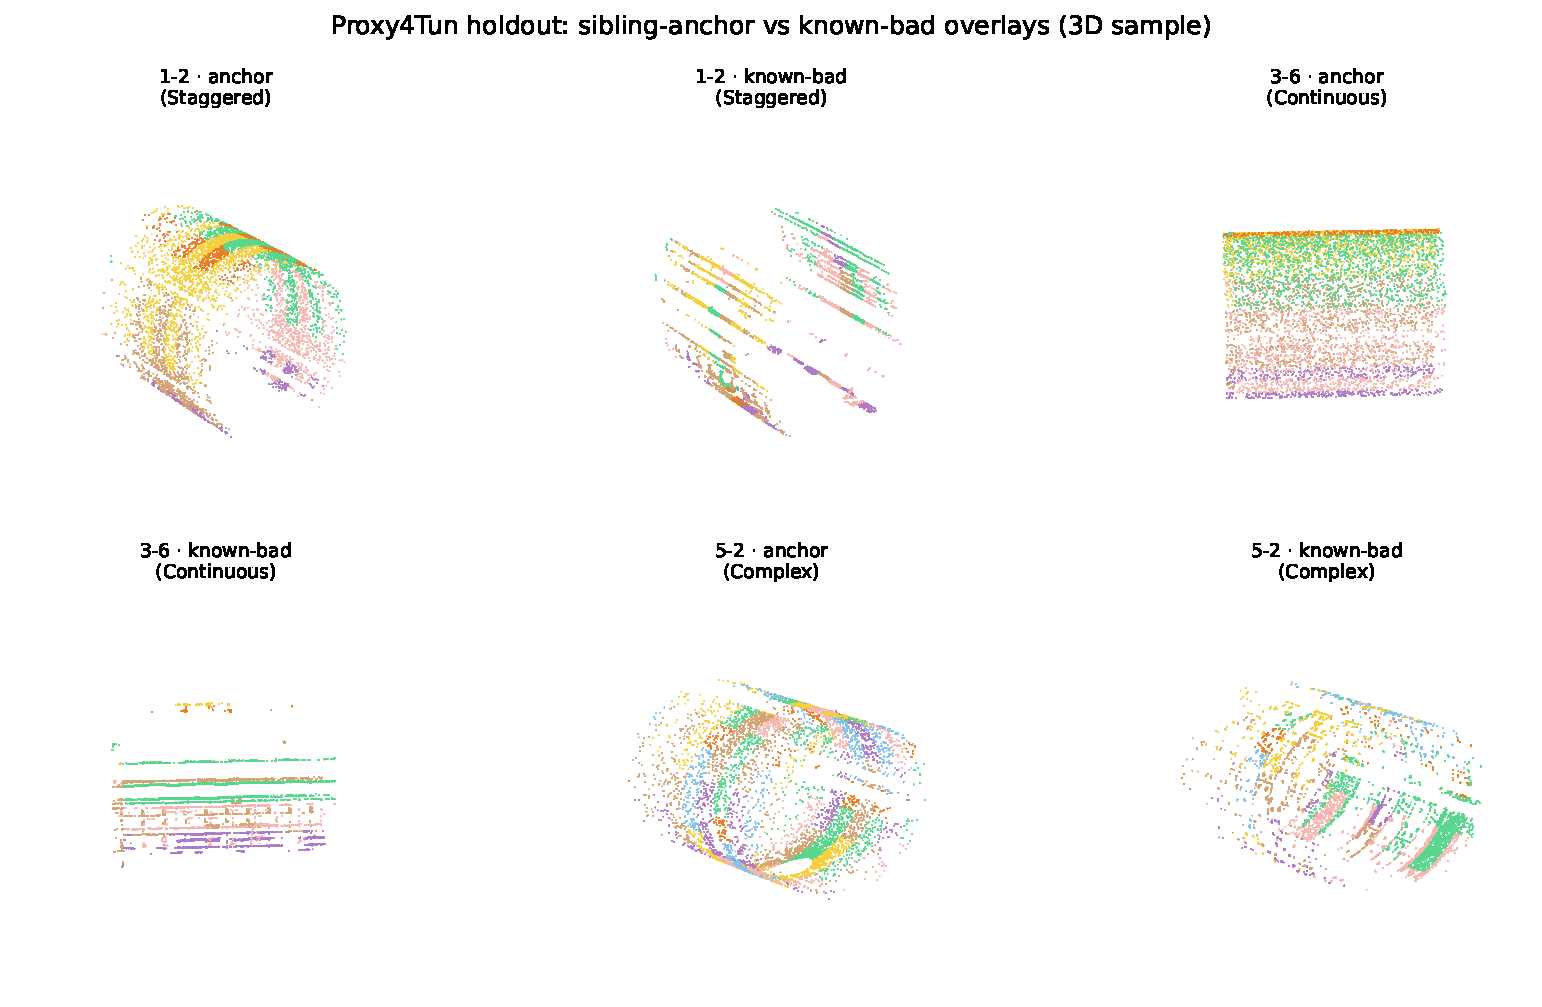
\includegraphics[width=0.98\textwidth]{figs/proxy4tun_3d_anchor_vs_bad.pdf}
\caption{Qualitative 3D samples on held-out subsets (staggered, continuous,
complex). Top: sibling-anchor configurations. Bottom: family known-bad
configurations. Points coloured by predicted segment class (background
suppressed). The proxy separates these regimes without access to labels.}
\label{fig:3d-anchor-bad}
\end{figure*}

\textbf{Blocking low-quality runs.} Used as an alarm at threshold
$\tau = 0.495$, the proxy flags all 27 known-bad runs while raising no false
alarms on the 27 sibling-anchor runs (Table~\ref{tab:holdout-fidelity});
anchor-versus-bad ranking is correct on all 27 subset pairs
(Fig.~\ref{fig:3d-anchor-bad} shows representative pairs). Given the size of
the flagged set we report raw counts rather than rates; the operating point
was fixed before holdout scoring and not tuned on the test subsets.

In practical terms, scoring a run is a five-feature linear evaluation over
artifacts the pipeline has already produced --- effectively free relative to
the pipeline run itself, and requiring no annotation. This is what makes the
proxy usable as an always-on acceptance gate and as a between-round selection
signal for iterative refinement (Section~\ref{sec:poc-verification}).

\subsection{Ablation analysis}\label{sec:proxy-ablation-results}

To isolate the contribution of each feature group, Table~\ref{tab:ablation-results}
and Fig.~\ref{fig:ablation-variants} report each ablation condition
(Table~\ref{tab:proxy-ablation}) under two regimes: training fit (Spearman
$\rho$ on the 120 calibration trials) and leave-one-family-out (LOLO)
cross-validation, in which the model is fitted on two anchors and evaluated on
the third. The LOLO columns are the ones that matter for deployment, since
they measure transfer to a family the model has not seen.

\begin{figure*}[t]
\centering
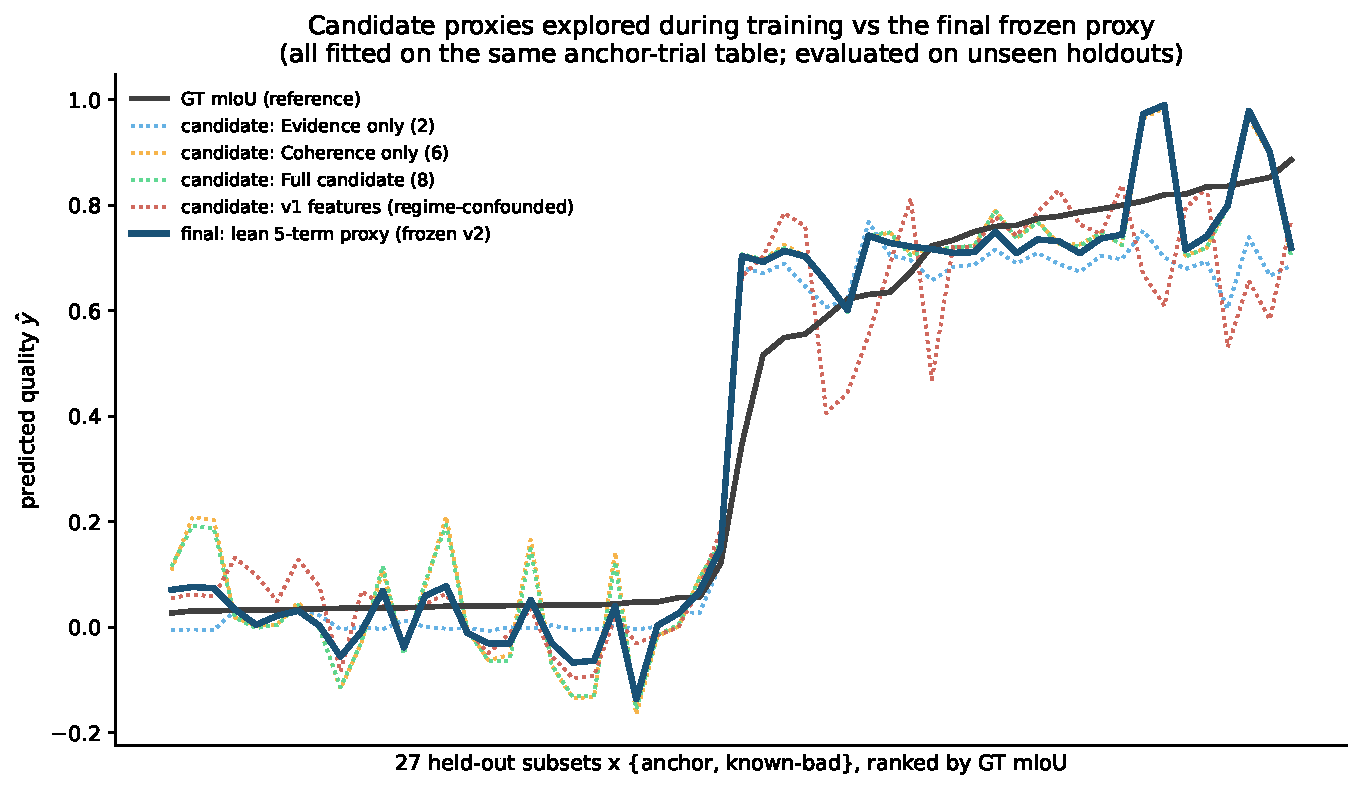
\includegraphics[width=0.85\textwidth]{figs/proxy_variants.pdf}
\caption{Feature-set ablation of the proxy: candidate variants (evidence-only
P(e), coherence-only P(c), combined P(e+c)) versus the final frozen lean
P(e+c), all fitted on the same 120-trial table and evaluated on the 54 unseen
holdout runs ranked by GT mIoU. The lean five-feature model tracks the GT
ordering most closely; pruning, not combination alone, delivers the best
cross-family transfer.}
\label{fig:ablation-variants}
\end{figure*}

\begin{table*}[t]
\caption{Proxy feature-set ablation. Train $\rho$ is the Spearman correlation
on the 120 calibration trials; LOLO columns report leave-one-family-out
cross-validation.}\label{tab:ablation-results}
\begin{tabular*}{\textwidth}{@{\extracolsep{\fill}} l c c c c @{}}
\toprule
Condition & \#Features & Train $\rho$ & LOLO $\rho$ & LOLO MAE \\
\midrule
P(e) (evidence only) & 4 & 0.682 & 0.429 & 0.405 \\
P(c) (coherence only) & 6 & 0.837 & 0.643 & 0.160 \\
P(e+c) (combined) & 10 & 0.876 & 0.537 & 0.346 \\
\quad $-$ \texttt{sam\_fill\_rate} & 9 & 0.700 & 0.198 & 0.415 \\
Stage-1 features only & 2 & 0.212 & $-$0.007 & 0.325 \\
\textbf{Lean P(e+c) (deployed)} & \textbf{5} & \textbf{0.853} & \textbf{0.717} & \textbf{0.156} \\
\bottomrule
\end{tabular*}
\end{table*}

\textbf{Evidence alone is insufficient.} The evidence-only proxy P(e) tracks
artifact quality (depth-map completeness, denoising retention, stage-1
geometry) but correlates only weakly with final segmentation quality
($\rho = 0.682$ train, 0.429 LOLO). Artifact quality is a necessary but not
sufficient condition: a run can produce a clean depth map and still assign
segment labels with the wrong structure.

\textbf{Coherence carries most of the signal.} The coherence-only proxy P(c)
reaches $\rho = 0.837$ on training trials and generalises markedly better than
evidence alone (LOLO MAE 0.160 vs.\ 0.405). Features describing the
\emph{form} of the result --- segment fill rate, class balance, and K-row
detection consistency --- are the primary carriers of quality information,
led by \texttt{sam\_fill\_rate}: removing this single feature from the
combined set collapses cross-family transfer ($\rho_{\text{LOLO}}$ 0.537
$\rightarrow$ 0.198).

\textbf{Combination helps in-sample; pruning is what makes it transfer.} The
full combined set P(e+c) achieves the best training fit ($\rho = 0.876$) but
generalises \emph{worse} than coherence alone (LOLO $\rho = 0.537$),
indicating that the weaker features overfit anchor-specific regularities.
Leave-one-out pruning to the five-feature lean set restores and surpasses
both: LOLO $\rho = 0.717$ and MAE 0.156, the best transfer of any condition.
The lean model is therefore not merely a parsimony choice --- pruning is
itself the mechanism that converts in-sample fit into cross-family
generalisation. The influence of the retained coefficients is analysed in
Section~\ref{sec:sensitivity}.

\textbf{Stage-1 features do not survive pruning.} Included as evidence
candidates for the first time in this campaign, the two stage-1 audit features
(centreline residual, orientation agreement) carry almost no standalone signal
($\rho = 0.212$ train, LOLO $\approx 0$) and are pruned from the lean set.
This is an honest boundary of the current proxy: stage-1 geometry defects are
not visible to it, which is precisely the failure mode isolated by the 4-3
case study (Section~\ref{sec:poc-verification}) and the motivation for stage-1
gating in future reflective agents.

\begin{table*}[t]
\caption{Unified versus per-family lean P(e+c) on the 120-trial full-stage
table (same five features; 40 trials per family). Holdout: 27 subsets, 54
scored runs.}\label{tab:unified-vs-perfamily}
\begin{tabular*}{\textwidth}{@{\extracolsep{\fill}} l c c c c @{}}
\toprule
Model & MAE & Spearman $\rho$ & Rank & Alarm P/R \\
\midrule
Lean unified (pooled) & 0.071 & 0.848 & 27/27 & 1.00 / 1.00 \\
Lean per-family & 0.057 & 0.872 & 27/27 & 1.00 / 0.96 \\
\bottomrule
\end{tabular*}
\end{table*}

\textbf{Unified versus per-family.} Refitting the same lean features as three
family-specific Ridge models (40 trials each) versus one pooled model
(120 trials) yields Table~\ref{tab:unified-vs-perfamily}. Per-family
calibration edges the pooled model on absolute fidelity (MAE 0.057 vs.\ 0.071;
$\rho$ 0.872 vs.\ 0.848), while both achieve perfect anchor-versus-bad ranking
(27/27). The pooled model retains perfect alarm recall (1.00 vs.\ 0.96; one
missed low-mIoU run under per-family thresholds). We therefore deploy the
unified model: the fidelity gap is small ($+$0.014 MAE), a single calibration
is operationally simpler, and alarm recall is undiminished. Earlier unbalanced
per-family fits (14/35/14 rows) had already shown that starving family-specific
models harms alarm recall more than it helps MAE; the balanced 40/family design
closes the MAE gap but does not overturn the case for pooling.

\subsection{Proof-of-concept verification: the proxy as a self-refinement signal}\label{sec:poc-verification}

\begin{figure*}[t]
\centering
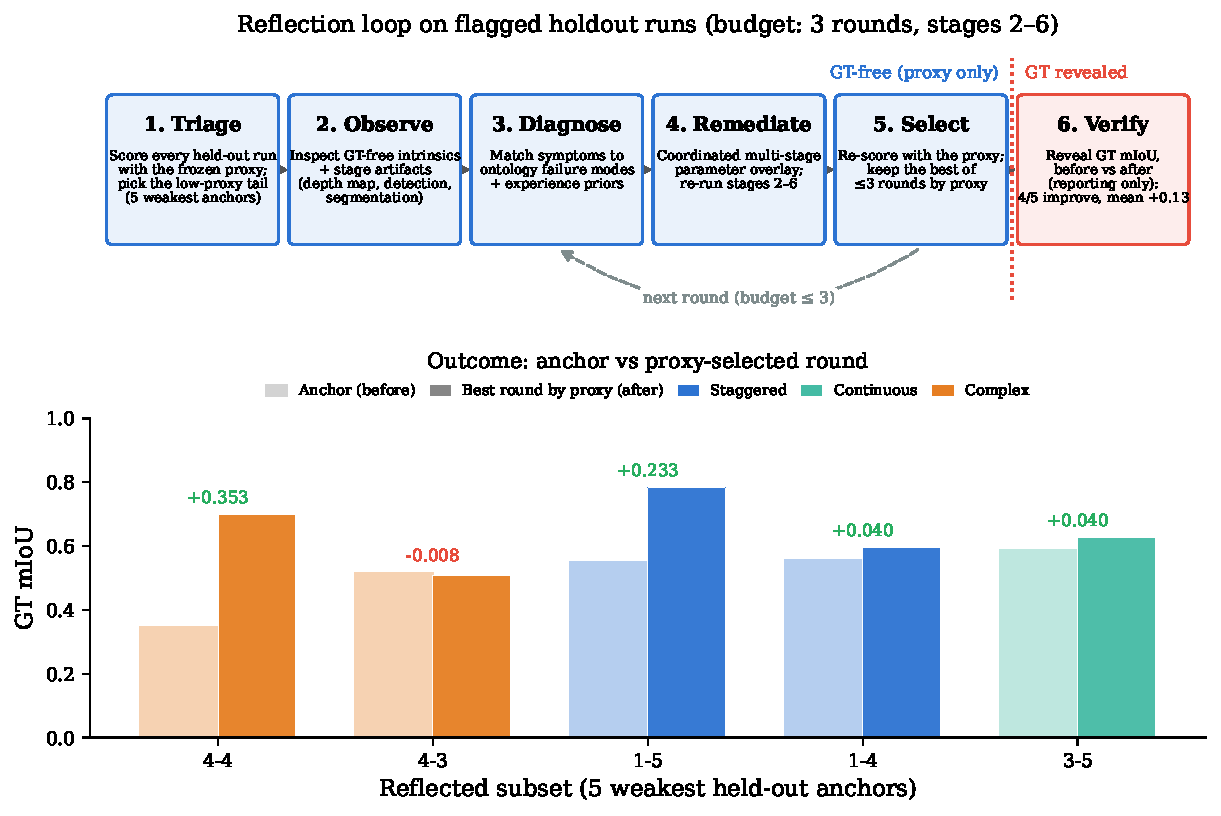
\includegraphics[width=0.95\textwidth]{figs/reflection_workflow.pdf}
\caption{PoC reflection loop on flagged holdout runs (budget: three rounds,
stages 2--6). Top: the GT-free loop --- triage by frozen proxy, artifact
observation, ontology-based diagnosis, bounded multi-stage remediation, and
proxy-based selection --- with GT revealed only at final verification.
Bottom: outcome per reflected subset, anchor versus the proxy-selected round.}
\label{fig:poc-workflow}
\end{figure*}

The final experiment tests whether the frozen proxy can drive a label-free
refinement loop (Fig.~\ref{fig:poc-workflow}). Each of five subsets is first
processed with its family anchor parameters and scored by the proxy. Runs
scoring at or above the acceptance threshold ($\tau = 0.7$) would be accepted
directly; below it, an LLM agent inspects the GT-free intrinsics and
artifacts, diagnoses deviations via the tunnel ontology, and proposes a
bounded multi-stage parameter overlay. Each round is re-scored by the proxy,
and after at most three rounds the highest-proxy configuration is retained.
The acceptance threshold is a deliberately conservative operating point on
the proxy score, distinct from the low-quality alarm threshold
($\tau = 0.495$) validated in Section~\ref{sec:main-results}: the former asks
``is this run good enough to ship without refinement?'', the latter ``is this
run bad enough to flag?''. Ground-truth mIoU is revealed only at final
evaluation and never enters the loop. Given the small sample ($n = 5$), we
report results per case and draw no statistical conclusions beyond
demonstrated feasibility.

\begin{table}[ht]
\caption{Proof-of-concept self-refinement: best-of-three reflection rounds
selected by proxy score, evaluated against ground truth only
afterwards.}\label{tab:poc-results}
\begin{tabular*}{\tblwidth}{@{} l c c c c @{}}
\toprule
Subset & Anchor mIoU & Selected mIoU & $\Delta$mIoU & Improved \\
\midrule
4-4 & 0.347 & 0.700 & $+$0.353 & yes \\
1-5 & 0.549 & 0.782 & $+$0.233 & yes \\
1-4 & 0.556 & 0.596 & $+$0.040 & yes \\
3-5 & 0.588 & 0.628 & $+$0.040 & yes \\
4-3 & 0.516 & 0.508 & $-$0.008 & no \\
\bottomrule
\end{tabular*}
\end{table}

\textbf{Selection by proxy improves four of five subsets.}
Table~\ref{tab:poc-results} summarises the campaign. Selecting the round with
the highest proxy score improves ground-truth mIoU on 4/5 subsets, with gains
from $+$0.040 to $+$0.353; the largest gain (subset 4-4, 0.347
$\rightarrow$ 0.700) doubles segmentation quality on a complex tunnel whose
anchor configuration under-detected ring boundaries. In each improved case
the round selected by proxy also improved ground-truth mIoU.

\begin{figure*}[t]
\centering
\begin{subfigure}{0.32\textwidth}
\centering
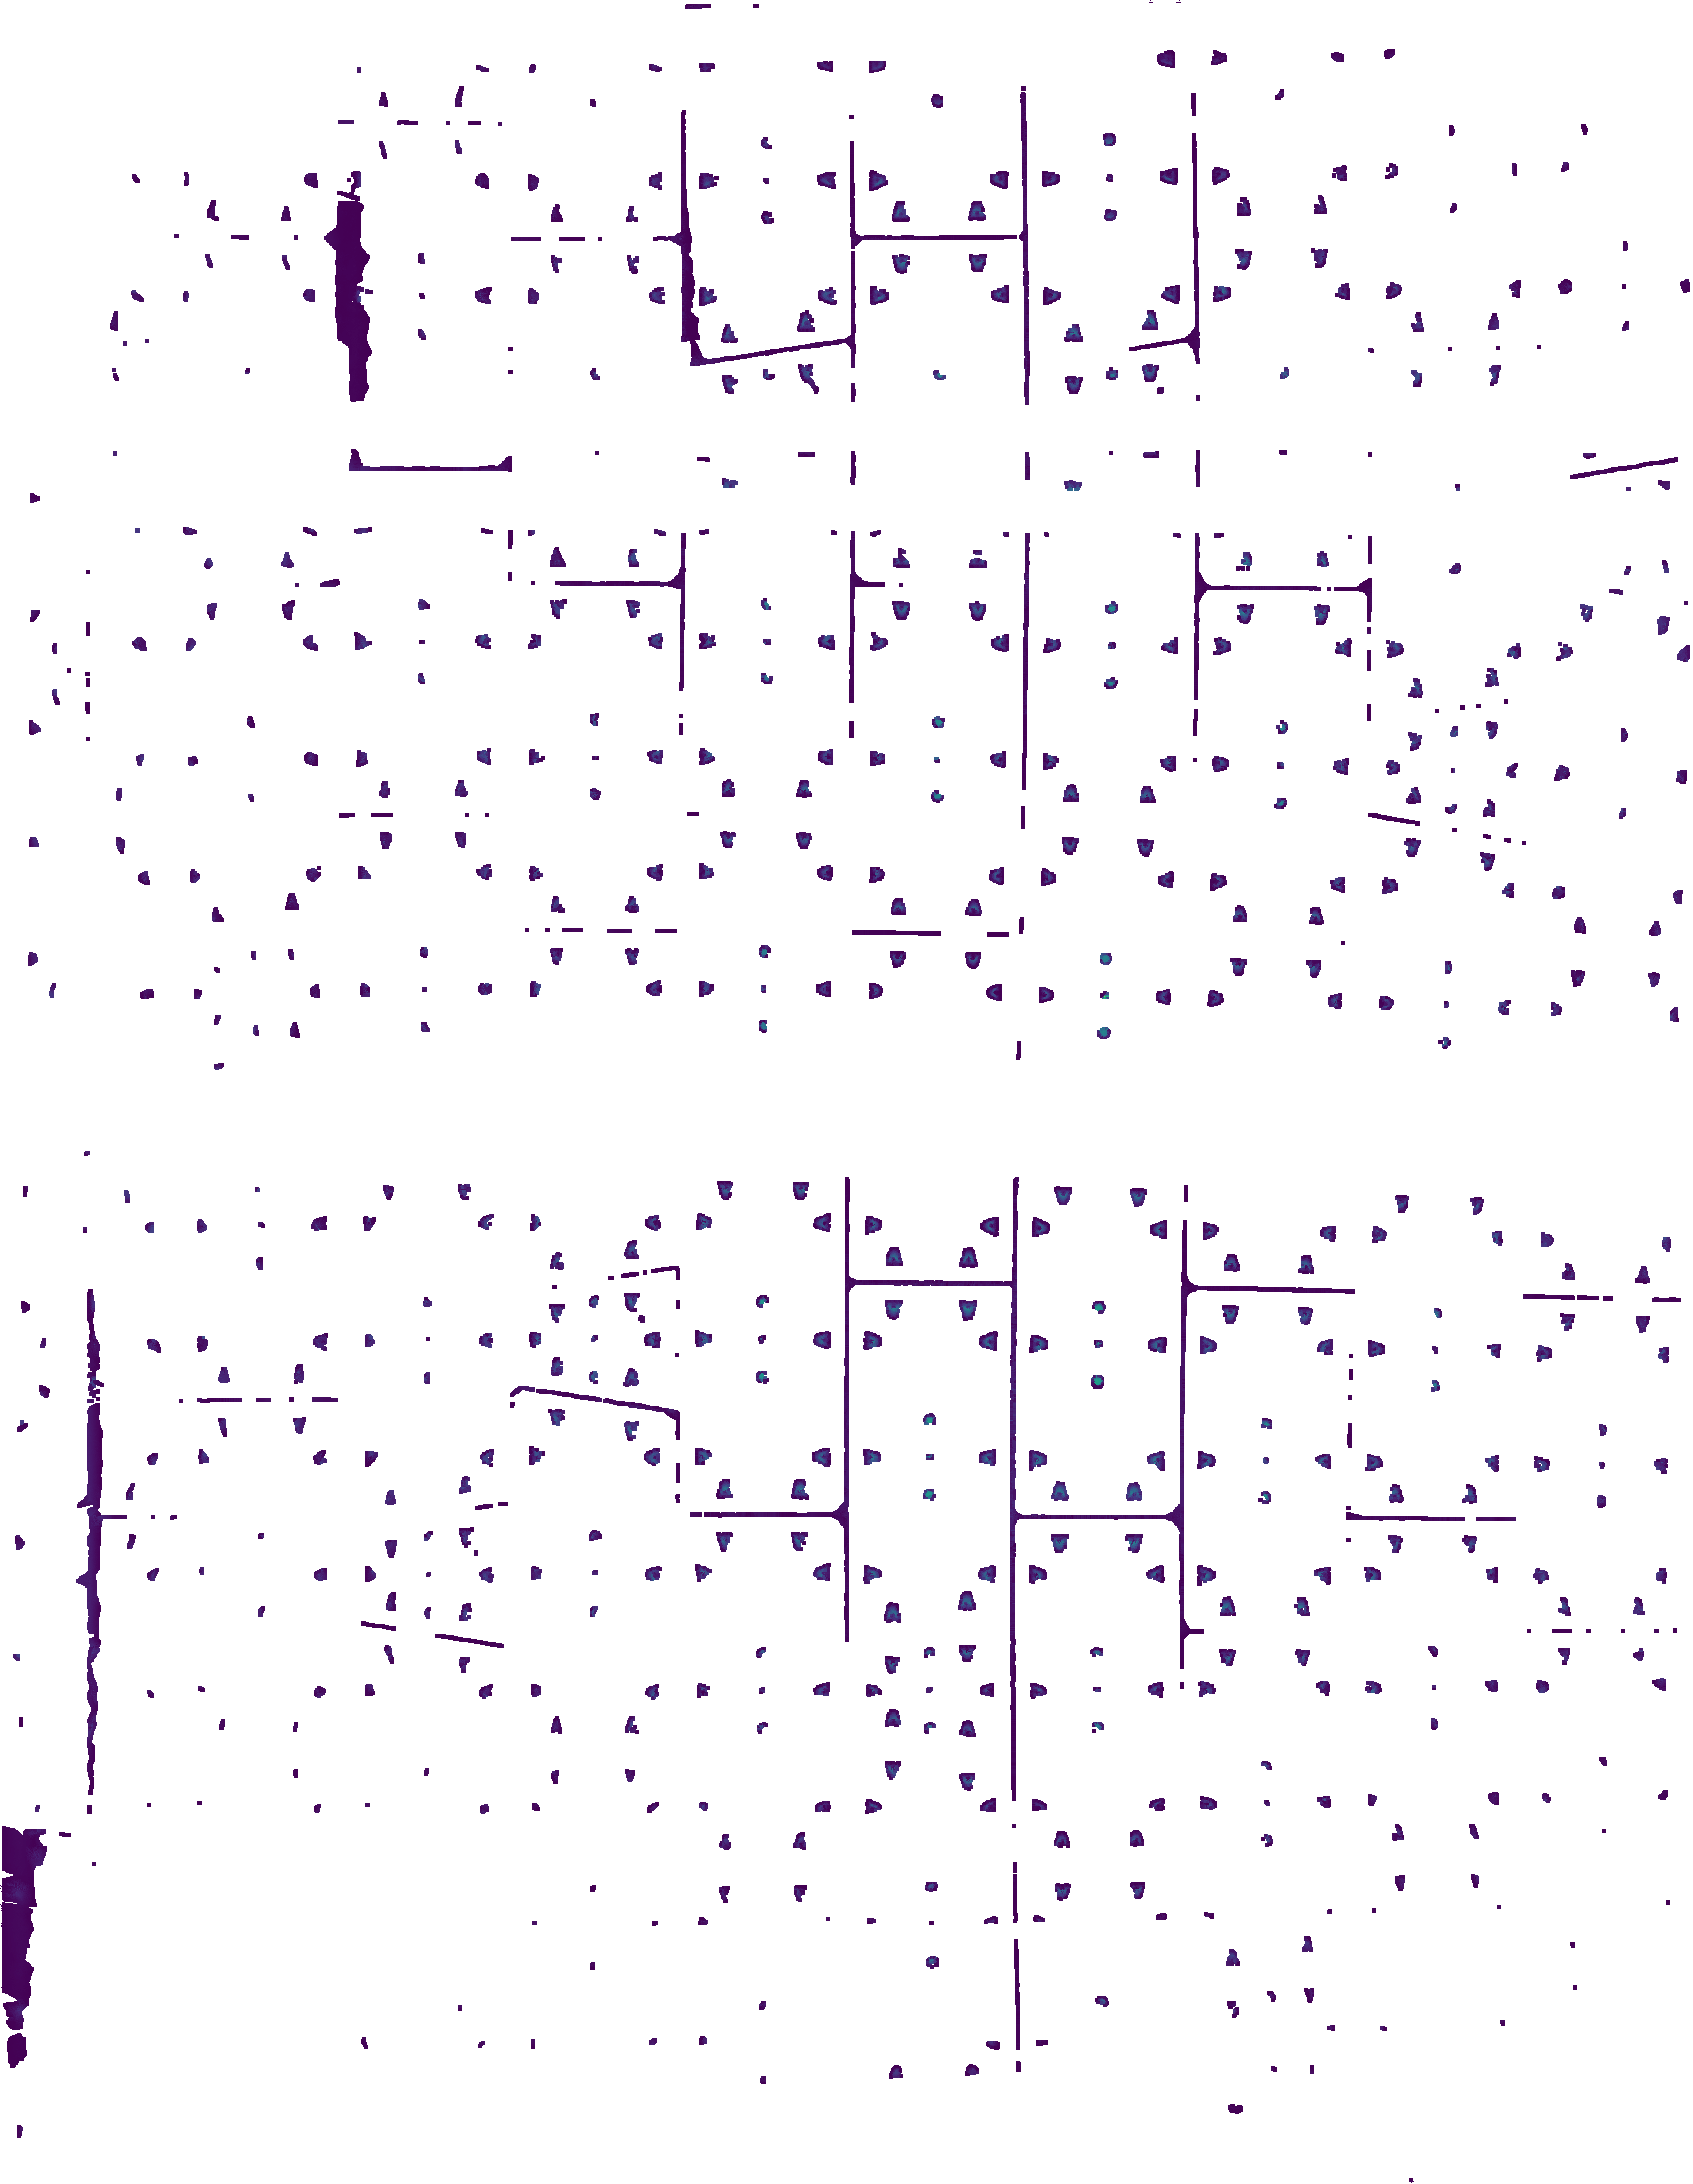
\includegraphics[width=\textwidth]{figs/5-1/low_depth_map.png}
\par\smallskip
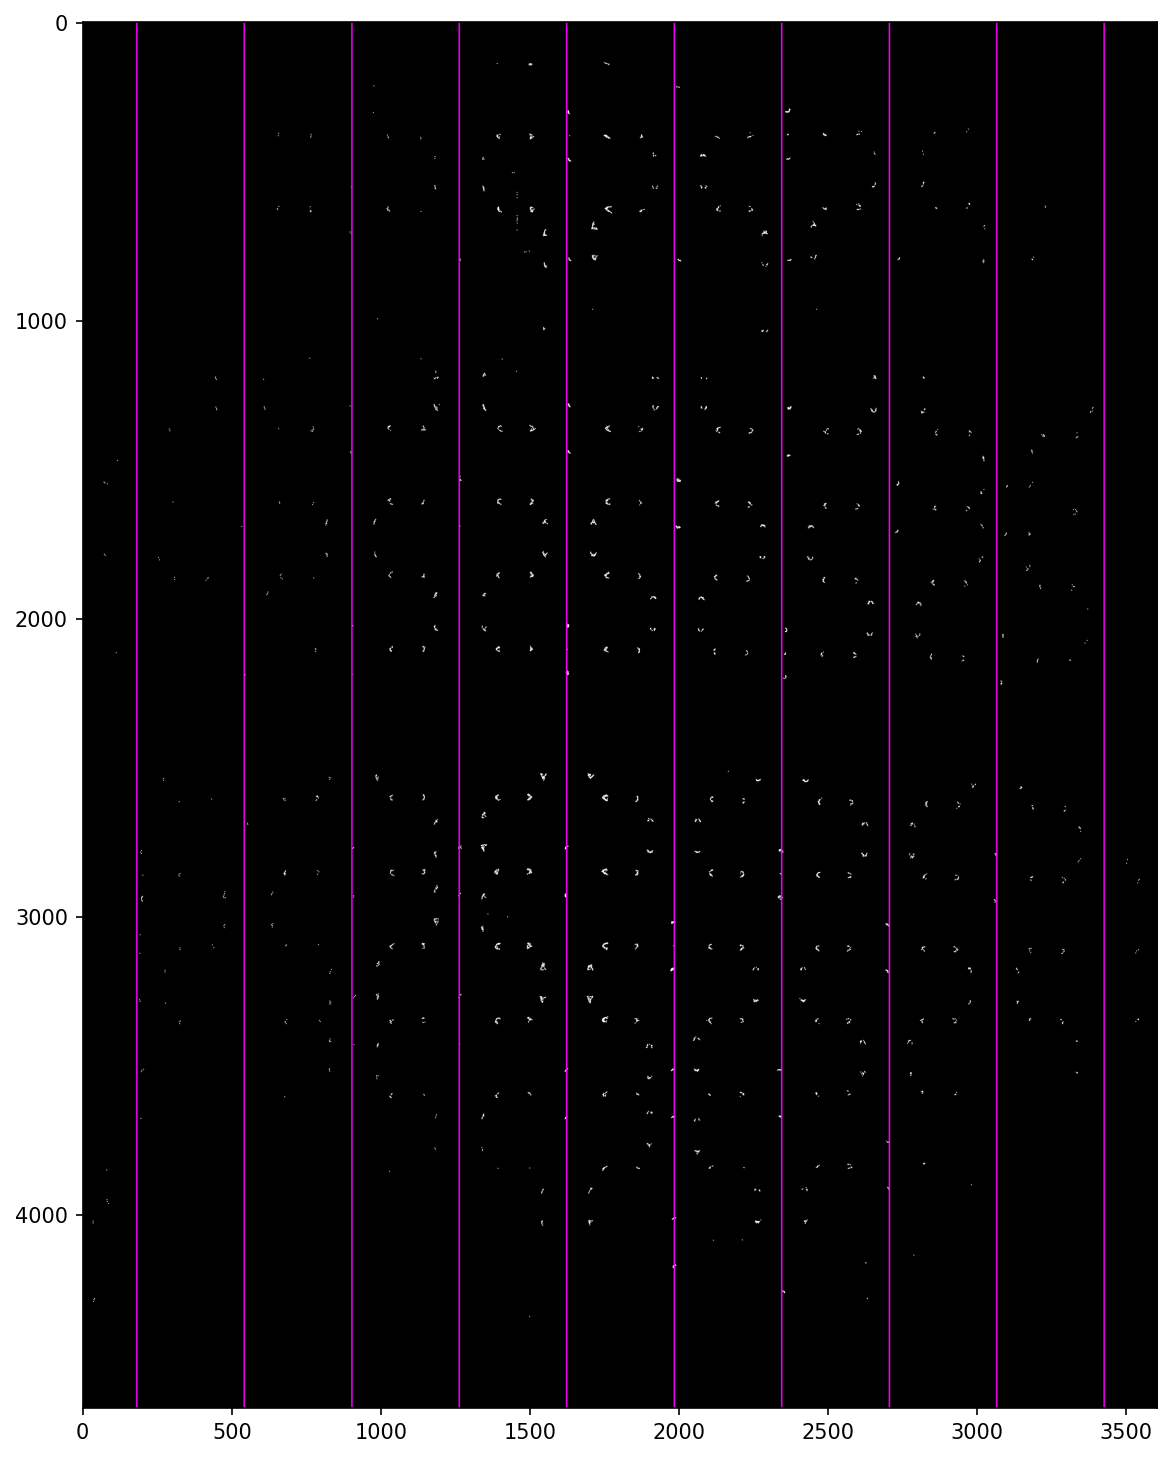
\includegraphics[width=\textwidth]{figs/5-1/low_detected_lines.png}
\par\smallskip (a) Low quality
\end{subfigure}
\hfill
\begin{subfigure}{0.32\textwidth}
\centering
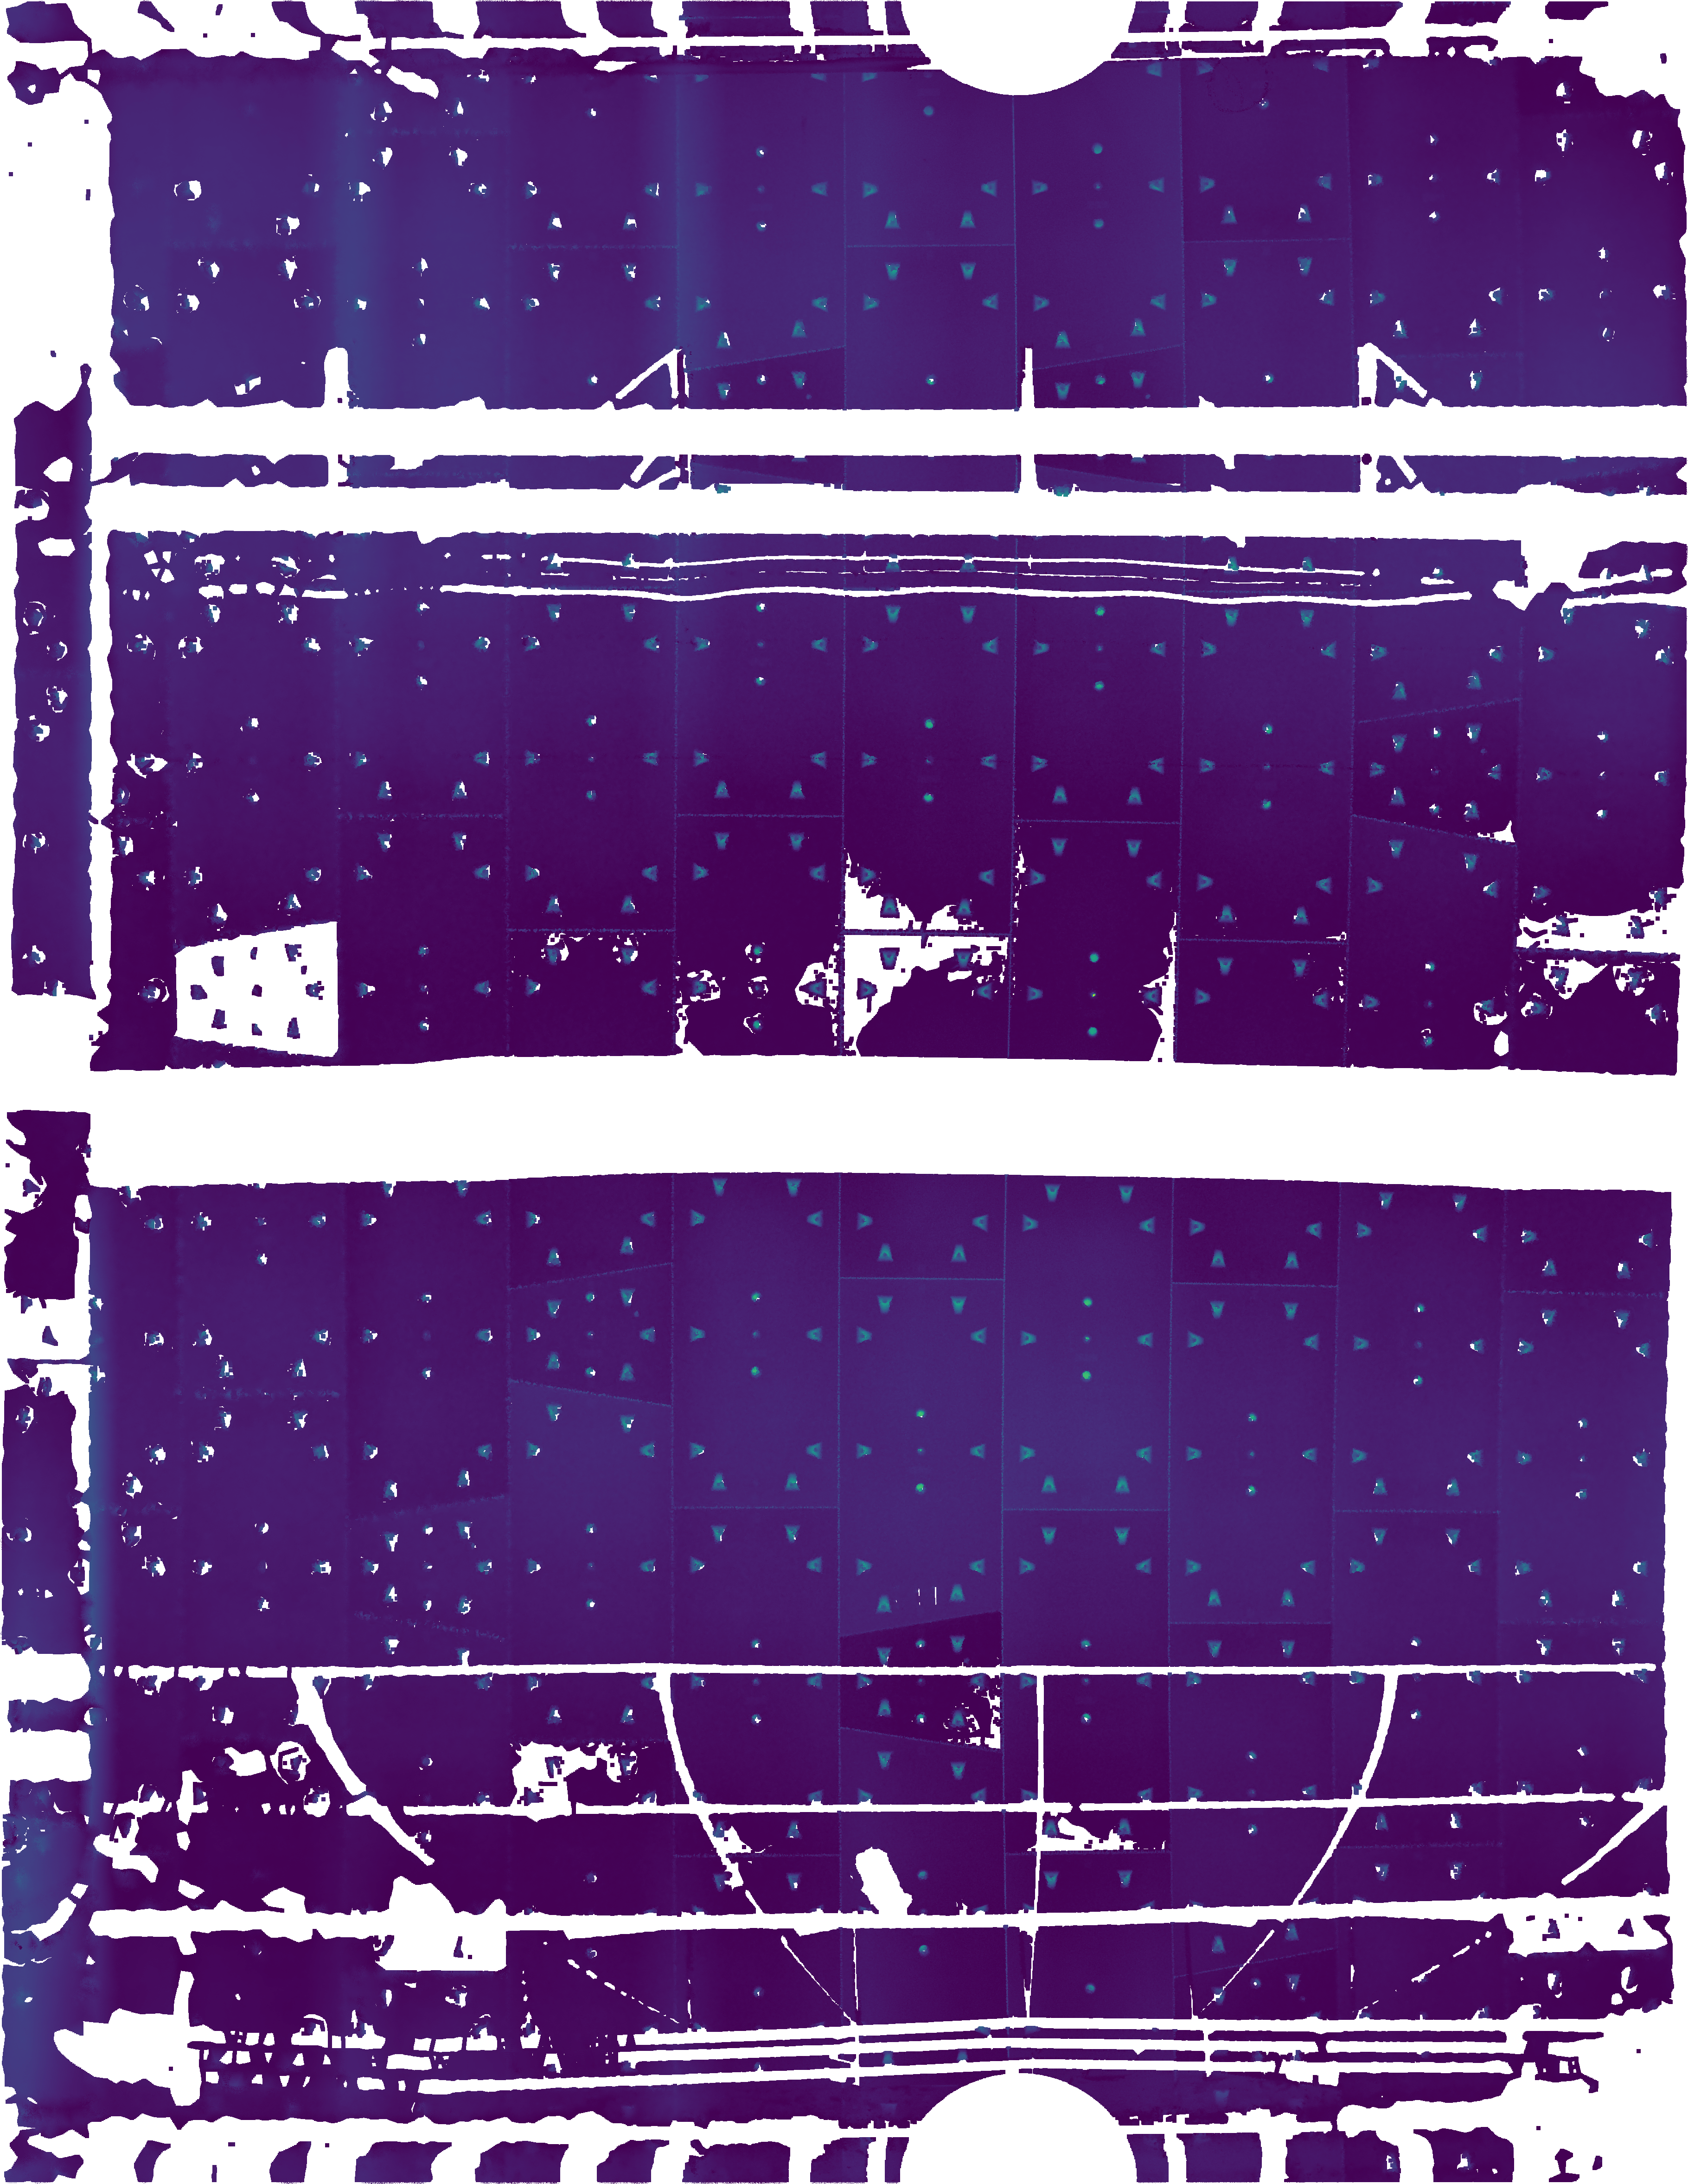
\includegraphics[width=\textwidth]{figs/5-1/mid_depth_map.png}
\par\smallskip
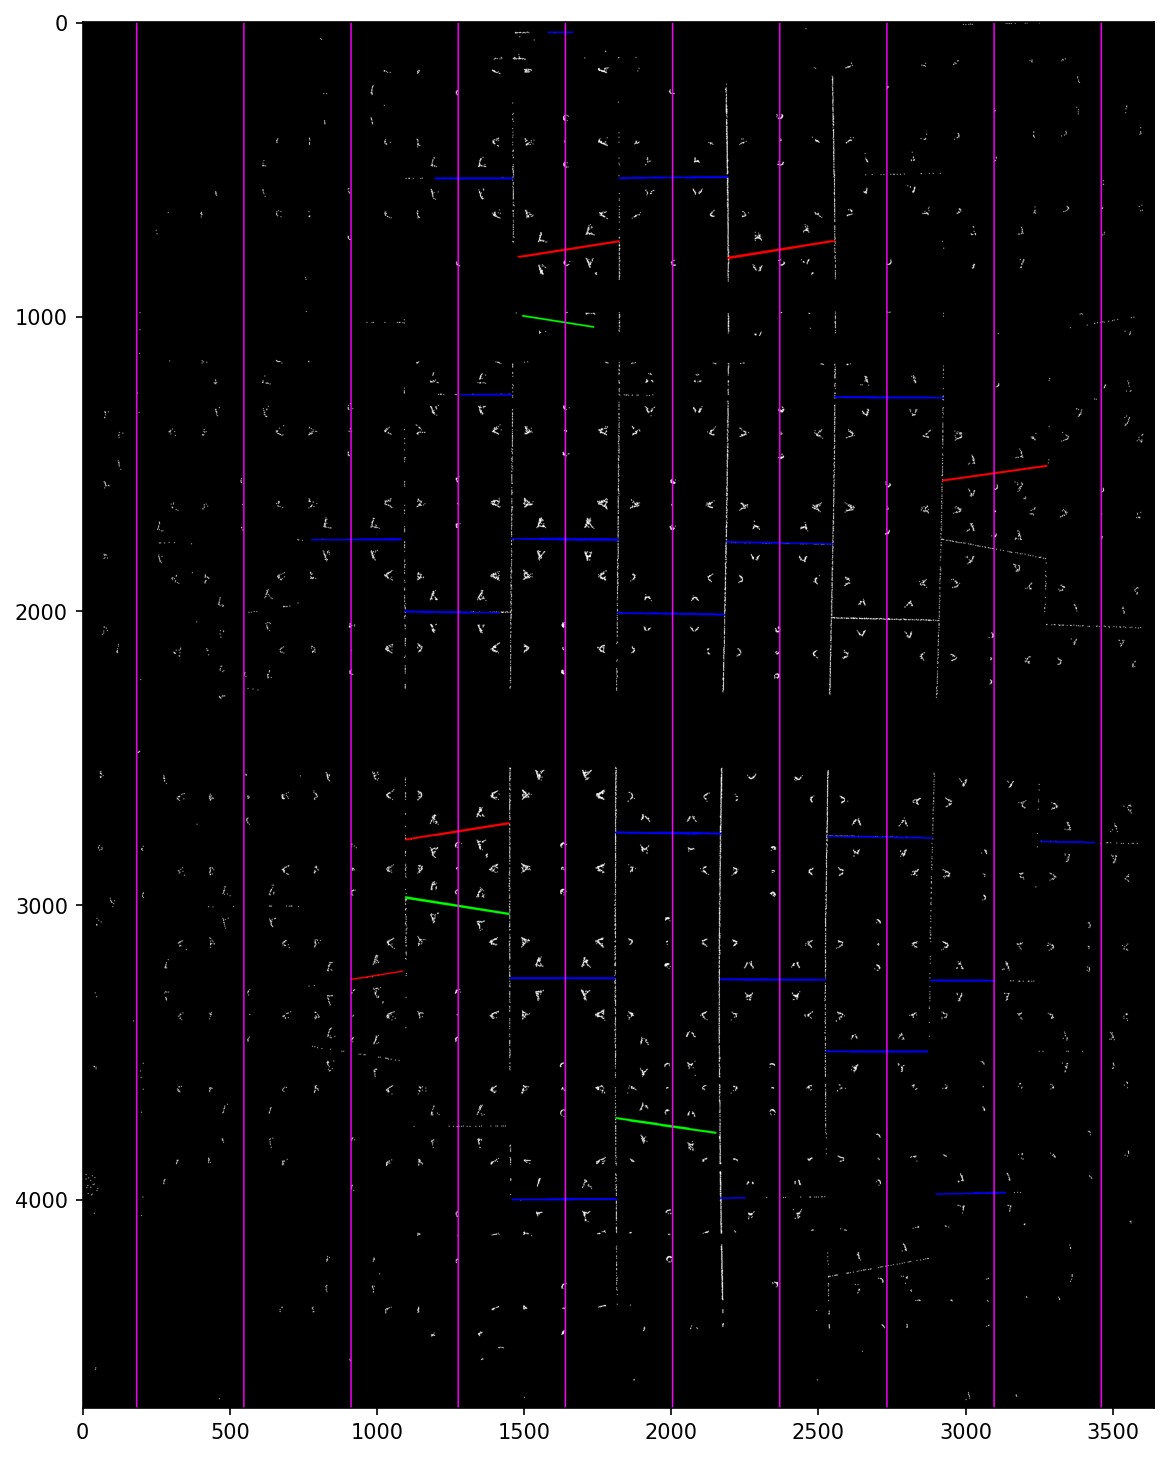
\includegraphics[width=\textwidth]{figs/5-1/mid_detected_lines.png}
\par\smallskip (b) Medium quality
\end{subfigure}
\hfill
\begin{subfigure}{0.32\textwidth}
\centering
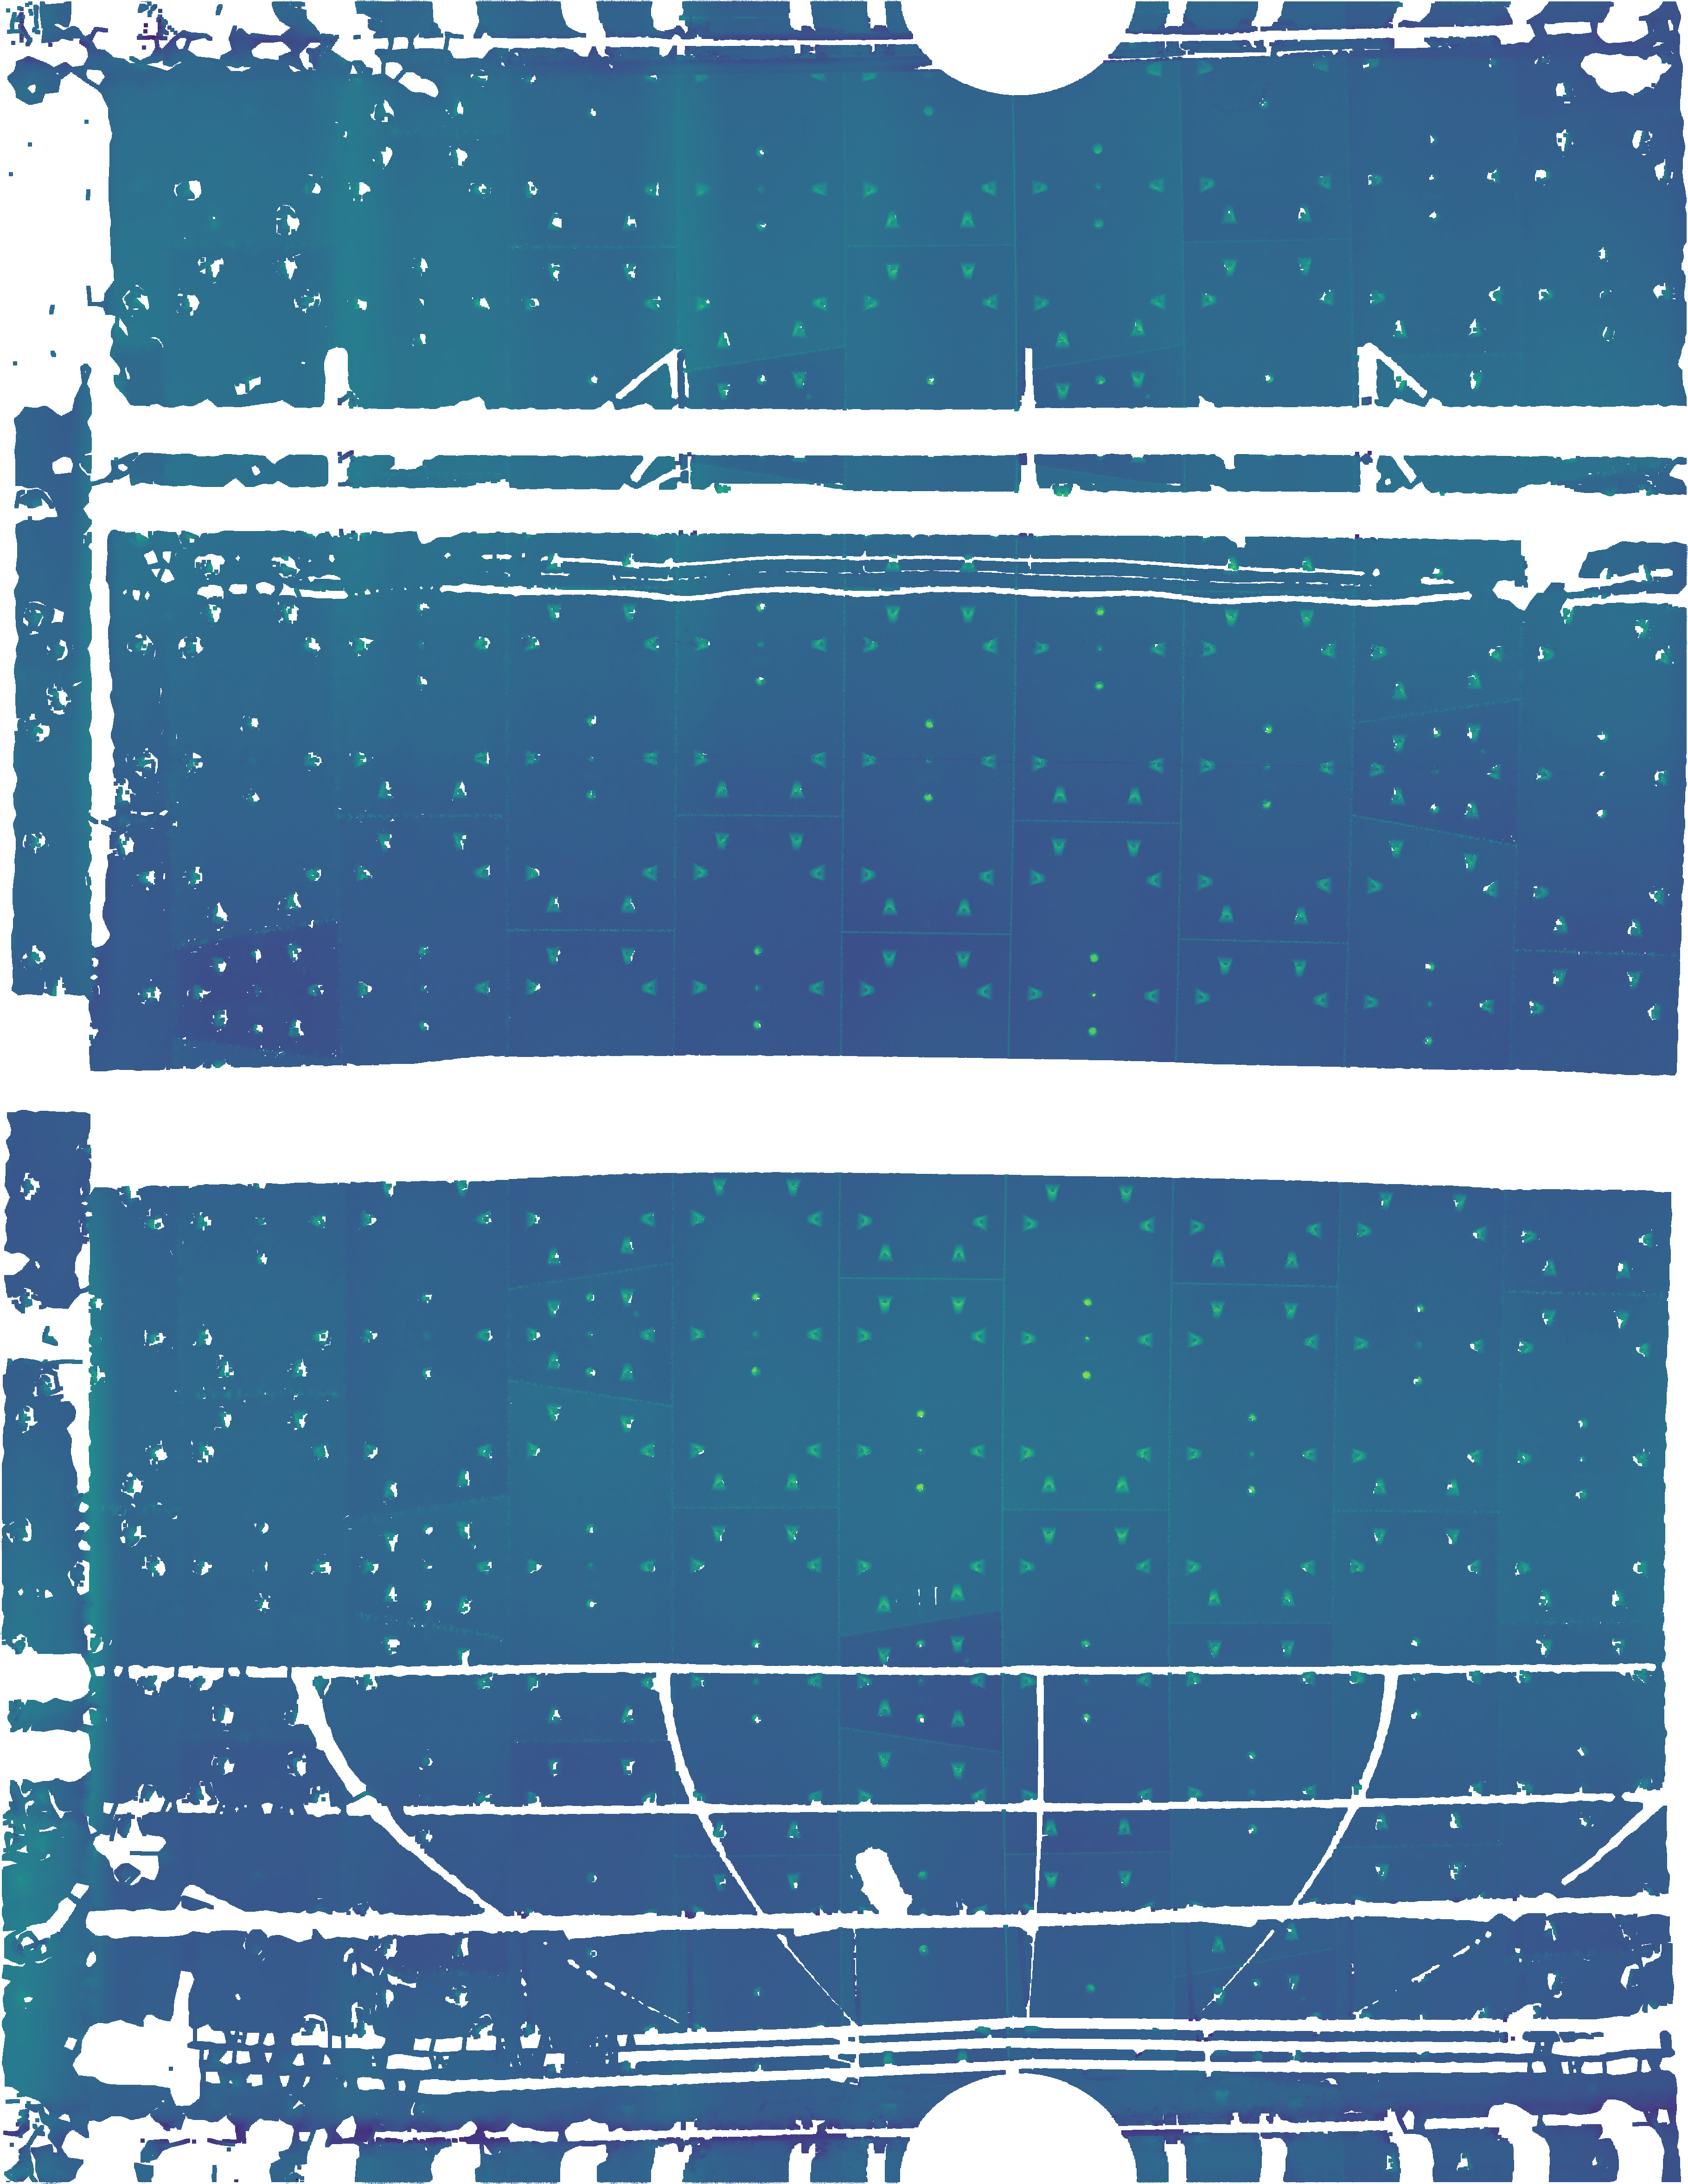
\includegraphics[width=\textwidth]{figs/5-1/best_depth_map.png}
\par\smallskip
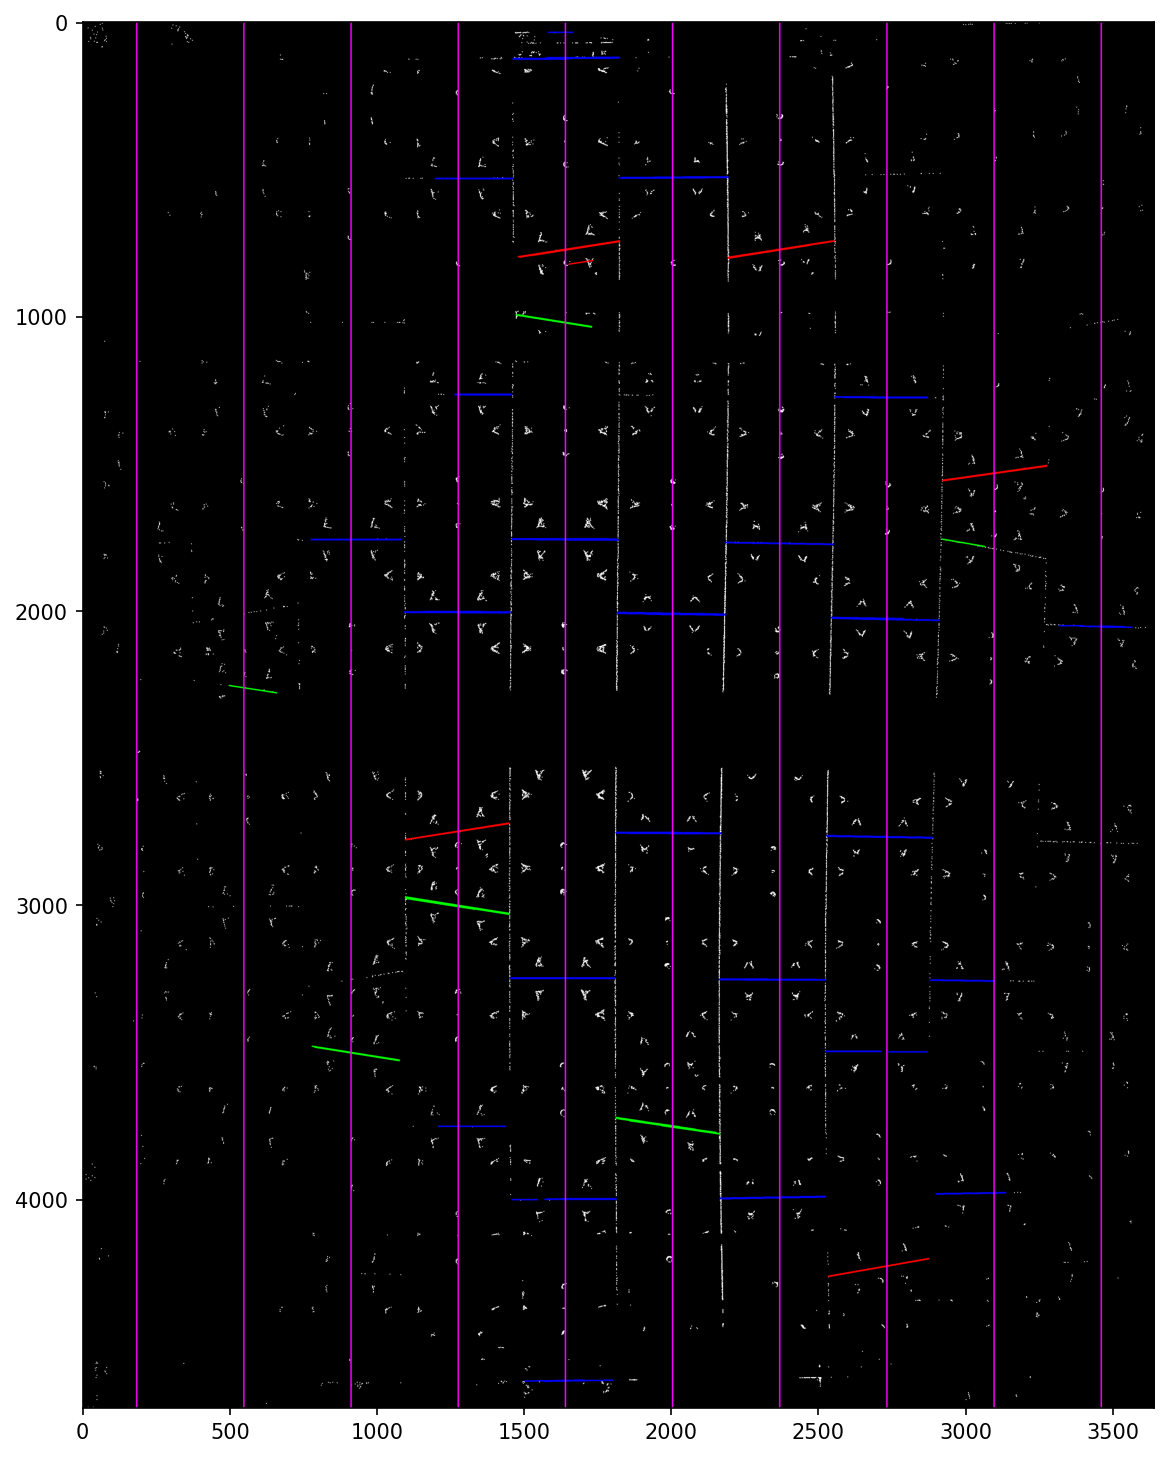
\includegraphics[width=\textwidth]{figs/5-1/best_detected_lines.png}
\par\smallskip (c) High quality
\end{subfigure}
\caption{What the proxy sees: unfolded depth maps (top) and detected joint
lines (bottom) for low-, medium-, and high-quality configurations of a
complex-family subset (5-1). Degraded configurations leave visible traces in
the artifacts --- incomplete depth coverage and irregular or missing joint
lines --- which the evidence and coherence features quantify without labels.}
\label{fig:poc-artifacts}
\end{figure*}

\textbf{Failure analysis: subset 4-3.} The one failure is diagnostic rather
than incidental. A ceiling probe over the stages 2--6 search space shows that
\emph{no} parameter overlay available to the reflection loop beats the anchor
on 4-3 (best manual configuration: $-$0.001; reflection best: $-$0.008): the
binding defect is the stage-1 centreline, whose recentring residual of
23.2\,cm distorts the unfolded geometry before any downstream parameter acts.
This quantity is invisible to the lean proxy --- substituting a healthy
residual into the 4-3 feature vector changes the prediction by exactly zero,
since the stage-1 candidates were pruned during feature ablation
(Section~\ref{sec:proxy-ablation-results}). When the loop is re-run with
stage~1 unlocked, changing the unfolding seed alone reduces the residual to
5.2\,cm and raises mIoU to 0.554 ($+$0.038 over the anchor), and all three
stage-1-aware rounds beat the anchor. The proxy thus delimits its own scope:
it reliably scores what the depth-map and segmentation artifacts reveal
(Fig.~\ref{fig:poc-artifacts}), and the 4-3 case identifies stage-1 geometry
auditing as the concrete extension required for a fully reflective agent.

\textbf{Scope of the claim.} This PoC is intended to demonstrate the proxy's
potential as a self-refinement signal for reflective LLM agents or
reinforcement learning, not to establish a general adaptation method: the
subsets were chosen to span families and failure modes, the refinement budget
was fixed at three rounds, and no hyperparameters were tuned on the outcome.
Within that scope, the loop shows that a frozen, five-feature linear proxy is
informative enough to select better configurations without any deployment
labels --- and, through its one failure, shows precisely where richer stage-1
evidence is needed.

\subsection{Parameter sensitivity}\label{sec:sensitivity}

Because all features are standardised before the ridge fit, the frozen
coefficients (Table~\ref{tab:candidate-features}) are directly comparable and
constitute the sensitivity record of the deployed proxy. Written out, the
deployed model is a five-term linear formula over standardised features:

\begin{itemize}
\item \texttt{sam\_fill\_rate} ($+0.47$) is the dominant term. It measures the
fraction of points assigned a non-background segment label; healthy runs
label most of the lining surface, whereas collapsed configurations leave
large unlabelled regions, so a higher fill rate raises the predicted mIoU.
Its load-bearing role is confirmed independently by the ablation: removing
this single feature collapses cross-family transfer
($\rho_{\text{LOLO}}$ 0.537 $\rightarrow$ 0.198, Table~\ref{tab:ablation-results}).
\item \texttt{denoise\_retained\_ratio} ($-0.39$) is the strongest evidence
term, with a physically expected negative sign: effective denoising must
remove non-lining clutter, so a high retention ratio marks under-filtering
(clutter surviving the radial gates) and correctly predicts lower mIoU.
\item \texttt{depth\_nan\_ratio} ($-0.17$) penalises hollow depth maps: a
large fraction of empty pixels indicates that the projection lost surface
evidence, degrading everything downstream.
\item \texttt{det\_row\_gated} ($+0.13$) and \texttt{det\_row\_residual\_px}
($-0.11$) form a complementary K-row pair: the gate indicator rewards runs
in which the K-row verification produced usable evidence, while the residual
penalises detected rows that deviate from the design row pattern.
\end{itemize}

Two further sensitivity observations delimit the model. First, the pruned
features have provably zero influence: substituting an arbitrary value for a
pruned feature (e.g.\ the stage-1 centreline residual in the 4-3 case study,
Section~\ref{sec:poc-verification}) changes the prediction by exactly zero.
Sensitivity to stage-1 geometry is therefore not merely weak but structurally
absent, which is the proxy's one demonstrated blind spot. Second, the two
operating thresholds are decoupled and were fixed before holdout scoring: the
low-quality alarm at $\tau = 0.495$ (validated with 27/27 true positives and
zero false alarms, Section~\ref{sec:main-results}) and the deliberately
conservative PoC acceptance point at $\tau = 0.7$
(Section~\ref{sec:poc-verification}). Between these two thresholds the proxy
recommends refinement rather than acceptance or rejection, and shifting either
threshold trades review workload against risk in a manner an engineer can
audit directly on the linear score.

% ══════════════════════════════════════════════════════════════════════════
\section{Discussion}\label{sec:discussion}
% ══════════════════════════════════════════════════════════════════════════

The results support a mechanism-level claim: a frozen, five-feature linear model over stage-observable metrics can serve as a GT-free control signal for a multi-stage tunnel segmentation pipeline. Labels enter only once, at design-time calibration on Bayesian-exploration trials; every deployment-time decision---score, rank, accept, flag, or select between refinement rounds---is made from intermediate artifacts alone, and every decision is auditable because the model is linear with inspectable coefficients.

\subsection{Key findings}

Three findings organise the results. First, the quality signal lives in the \emph{form} of the result more than in the quality of the artifacts: coherence features (led by segment-mask fill rate) dominate both the ablation and the frozen coefficients, and the combined ten-feature set generalises \emph{worse} across families than coherence alone until leave-one-out pruning removes the anchor-specific features (LOLO Spearman 0.537 $\rightarrow$ 0.717). Pruning is therefore not a parsimony preference but the mechanism that converts in-sample fit into cross-family transfer. Second, one pooled model is the right deployment choice: per-family refits of the same lean features edge the pooled model on absolute fidelity (MAE 0.057 vs.\ 0.071) but lose alarm recall (0.96 vs.\ 1.00), and a single calibration is operationally simpler across the three lining families. Third, a well-calibrated intrinsic proxy enables practical, auditable self-refinement: instead of relying on a fixed parameter setting, the reflective loop searches bounded candidate adaptations and accepts only those the proxy endorses, allowing the pipeline to adapt to variations in diameter, segment count, and ring geometry while every decision remains reviewable.

For practice, the workflow implication mirrors the design: an engineer calibrates once per pipeline release---anchor selection, bounded exploration, ablation, freeze---and thereafter receives a per-run quality estimate and alarm at negligible cost. The PoC shows the same signal can drive refinement: selecting LLM-proposed overlays by proxy score improved four of five subsets without any label access. The single failure (4-3) is itself informative: the loop's ceiling probe and the proxy's provable insensitivity to the pruned stage-1 residual localise the defect to centreline geometry, turning a miss into a concrete specification for the next capability rather than an unexplained error.

\subsection{Comparison with state-of-the-art}\label{sec:positioning}

Comparisons here are about operating points, not accuracy leaderboards. Supervised 3D models on Seg2Tunnel report strong in-distribution accuracy~\cite{lin2024seg2tunnel} but require per-point labels and GPU retraining for each new lining family, and provide no deployment-time accept/refine/flag gate. Expert-tuned SAM4Tun reaches high accuracy on curated, per-case-tuned rings~\cite{ye2025sam4tun}, but a single fixed configuration transfers poorly off the reference and the pipeline emits no signal when it degrades. Relative to that static pipeline, Proxy4Tun adds an explicit accept/refine/flag channel without deployment labels. Relative to one-shot LLM parameter adapters, it adds a calibrated numeric critic, so refinement can be \emph{verified} rather than merely proposed. Relative to generic segmentation QC~\cite{valindria2017rca,fournel2021segmentationQC} and uncertainty estimation~\cite{gal2016dropout,lakshminarayanan2017deepEnsembles}, the feature set is specialised to cylindrical unfolding and segmental lining grammars, and the calibration cost is three labelled anchor tunnels rather than a labelled validation stream. BO remains offline experience generation~\cite{snoek2012practicalBO,garnett2023bayesianOptimization}; no labels or surrogates are queried at runtime.

\subsection{Limitations}\label{sec:limitations}

The frozen proxy has a demonstrated blind spot: stage-1 geometry. The two stage-1 audit features carried too little standalone signal to survive pruning, so centreline defects (as on subset 4-3) are invisible to the score; stage-1 gating or richer geometric evidence is required before the loop can be considered fully reflective. The proxy is also deliberately compact---five features and a linear map---which favours interpretability over expressiveness and can mis-rank candidates whose failure signatures fall outside the calibrated feature space. Calibration rests on one expert-tuned anchor per family, and transfer is demonstrated within Seg2Tunnel's three families under the SAM4Tun stage graph; different sensors, lining grammars, or pipelines require re-calibration, though the protocol itself (bounded exploration, ablation, permutation control, freeze) is pipeline-agnostic. The phase-coherence check is reliable only on regular linings, where a repeating stagger exists. Finally, the self-refinement PoC covers five subsets with a three-round budget and a single agent configuration; it demonstrates feasibility, not a validated adaptation method, and the bounded search is not exhaustive---finer-grained exploration, retrieval over accumulated refinement experience, or a learned proposal policy may identify further improvements.

% ══════════════════════════════════════════════════════════════════════════
\section{Conclusions}\label{sec:conclusions}
% ══════════════════════════════════════════════════════════════════════════

This paper presented Proxy4Tun, which calibrates a ground-truth-free quality proxy for segmental tunnel-lining segmentation from design-time Bayesian exploration and deploys it, frozen, as an auditable control signal. Space-filling exploration of the bounded parameter space around one expert-tuned anchor per lining family produced 40 labelled trials per family spanning healthy to degraded configurations; feature ablation over evidence and coherence metrics distilled these into a five-feature pooled Ridge proxy with a calibrated alarm. The main findings of this study are:

\begin{itemize}
\item On 27 held-out subsets (54 scored runs), the frozen proxy tracked GT mIoU with Spearman 0.848 and MAE 0.071, ranked the sibling anchor above a known-bad configuration on every subset, and flagged all 27 known-bad runs with zero false alarms.
\item Coherence features carry most of the quality signal, and leave-one-out pruning---not feature accumulation---delivers cross-family transfer; the deployed five-feature model outperforms the full ten-feature candidate set out of family.
\item A single pooled model matches per-family refits where it matters: per-family calibration gains 0.014 MAE but loses alarm recall, so one unified proxy serves all three lining families.
\item As a proof of concept, selecting LLM-proposed bounded parameter overlays by proxy score improved mIoU on four of five subsets ($+$0.040 to $+$0.353) without any deployment labels; the single failure was traced to a stage-1 centreline defect outside the proxy's feature scope.
\end{itemize}

The approach is limited by its stage-1 blind spot, its single-anchor-per-family calibration, and the scope of the PoC; absolute segmentation quality remains bounded by the underlying SAM4Tun stages. Future work will add stage-1 geometry auditing (residual and orientation gates) to close the demonstrated blind spot, extend the reflective agent to full campaigns across the holdout panel, use the frozen proxy as a reward signal for reinforcement-learning-based tuning, add uncertainty-aware abstention to the accept/refine/flag decision, and evaluate multi-anchor calibration for families with larger within-family variation. These results indicate that intrinsic, stage-observable metrics---calibrated once and frozen---can serve as an auditable control plane for foundation-model tunnel pipelines when ground truth is unavailable.

% ══════════════════════════════════════════════════════════════════════════
% Data availability, declarations, etc.
% ══════════════════════════════════════════════════════════════════════════

\section*{Data availability}

The source code, parameter snapshots, exploration-trial tables, and evaluation scripts will be released upon publication. The Seg2Tunnel dataset is publicly available~\cite{lin2024seg2tunnel}.

\section*{Declaration of competing interest}

The authors declare that they have no known competing financial interests or personal relationships that could have appeared to influence the work reported in this paper.

\section*{Declaration of generative AI use}

During this study, LLM agents (Fable 5 and GPT-5.6) were evaluated as the proposal mechanism of the proof-of-concept self-refinement loop. LLMs were also used for language editing and for improving manuscript structure. The authors reviewed and edited all content and take full responsibility for the content of the publication.

%\printcredits  % Uncomment if cas-dc supports it in your version

% ══════════════════════════════════════════════════════════════════════════
% Bibliography
% ══════════════════════════════════════════════════════════════════════════

% Natbib requires a BibTeX style; without it, citations stay as “?”
% NOTE: \balance can cause column-balancing artefacts in the reference list (e.g.,
% lines slipping into the footer area) with this class. Keep it off for the bibliography.
%\balance
\bibliographystyle{model1-num-names}
\bibliography{references}

\end{document}
